% (c) 2012 Tiziana Manca - tmanca@libero.it
% (c) 2012 -2014 Dimitrios Vrettos - d.vrettos@gmail.com

\chapter{Statistica descrittiva}

\section{Indagine statistica}
Il termine statistica significa \emph{scienza dello stato}. Questo termine venne usato per la prima volta nel~$XVI$ secolo
per indicare lo studio dei dati utili al governo degli stati prevalentemente relativi a fenomeni di carattere demografico (nascite, morti, ecc.).
Negli anni, la statistica si è estesa ai campi più disparati: fisica, psicologia, ricerca di mercato, indici di gradimento, sondaggi, meteorologia, \ldots
È nata essenzialmente con lo scopo di descrivere i fenomeni (statistica descrittiva), successivamente è divenuta uno strumento utile
anche per fare previsioni (statistica inferenziale). A grandi linee si può definire come la scienza che si occupa della raccolta e dell'analisi dei dati relativi
ad un certo gruppo di persone, animali o oggetti al fine di descrivere in maniera sintetica un fenomeno che li riguarda e fare eventualmente previsioni sul suo andamento futuro.

Ad esempio, la statistica cerca di rispondere a domande del tipo:
\begin{itemize*}
\item quanta acqua sarà necessaria in Italia fra~3 anni?
\item quanta corrente elettrica sarà necessaria per il fabbisogno nazionale fra~5 anni?
\item quale sarà il tasso di disoccupazione nazionale fra~1 anno?
\end{itemize*}

\begin{definizione}
L'insieme di elementi oggetto dell'indagine statistica è detta \emph{popolazione} o universo, mentre ciascun elemento della popolazione è detto \emph{unità statistica}.
\end{definizione}

Sono esempi di popolazione statistica gli abitanti di una città in un certo anno, i prezzi di un determinato bene, le temperature massime registrate
in una giornata in un particolare luogo, i ciclomotori circolanti in Italia, gli alunni di una scuola.

\begin{definizione}
Per ogni unità statistica si possono studiare una o più caratteristiche ed ognuna di tali caratteristiche costituisce un \emph{carattere} della popolazione oggetto
di indagine. I caratteri possono essere di tipo \emph{qualitativo} o \emph{quantitativo}.
Si definisce \emph{modalità} del carattere indagato ciascuno dei diversi modi in cui esso può presentarsi.
\end{definizione}

Sono esempi di carattere qualitativo il colore degli occhi, il colore dei capelli, il tipo di scuola frequentato, il gradimento di un certo programma televisivo.
Le modalità di un carattere qualitativo sono espresse mediante nomi o aggettivi.
I caratteri qualitativi sono a loro volta suddivisi in \emph{ordinabili}, cioè può essere definita una relazione di ordine tra essi (per ogni coppia di elementi si può stabilire quale dei due è il primo e quale il secondo -- es.~il tipo di scuola frequentato è ordinabile a partire dalla scuola dell'infanzia fino alla laurea,
il gradimento di un programma televisivo è ordinabile a partire dalla completa mancanza di gradimento fino al gradimento massimo) e \emph{non ordinabili} o \emph{sconnessi}
(es.~colore degli occhi, colore dei capelli).

Sono invece caratteri quantitativi l'età, l'altezza, il numero di auto prodotte da una fabbrica, \ldots, ovvero le modalità di un carattere quantitativo sono espresse mediante numeri.
I caratteri quantitativi possono essere di tipo \emph{discreto}, quando assumono solo valori puntuali, oppure di tipo \emph{continuo}, quando possono assumere
tutti gli infiniti valori compresi in un determinato intervallo. Sono esempi di caratteri quantitativi discreti il numero di figli in una famiglia,
i pezzi prodotti in una catena di montaggio; sono esempi di caratteri quantitativi continui l'altezza di una persona, il peso di una persona, la lunghezza di un fiume.

L'indagine statistica può riguardare l'intera popolazione (in tal caso si parla di \emph{censimento}) oppure solo una sua parte (in tal caso si parla di \emph{indagine a campione}).
Supponiamo di voler effettuare un'indagine relativa alle persone che fumano in Italia. Il fenomeno collettivo in esame è il fumo, la popolazione di riferimento
è costituita dalla popolazione italiana in età adulta, l'unità statistica è rappresentata da ogni cittadino oggetto dell'indagine, i caratteri oggetto
dell'indagine possono essere ``fumatore/{}non fumatore'', ``numero di sigarette fumate'', che cosa si fuma (es.~ pipa, sigaro, sigaretta). Data l'elevata numerosità
della popolazione di riferimento la tipologia di indagine preferibile è quella a campione.

A sua volta, l'indagine a campione può essere effettuata su un \emph{campione casuale}, quando si scelgono a caso i campioni all'interno della popolazione o
su un \emph{campione stratificato}, quando si suddivide la popolazione in \emph{classi} o \emph{strati} senza specifici criteri e per ogni strato si prende a caso un campione.

\ovalbox{\risolvi \ref{ese:A.1}}

\section{Fasi di un'indagine statistica}
\begin{definizione}
Dato un carattere oggetto di rilevazione, si definisce \emph{frequenza} il numero delle unità statistiche su cui una sua modalità si presenta.
\end{definizione}

Affinché un'indagine statistica sia rigorosa (e quindi garantisca un'elevata affidabilità) è necessario che sia strutturata secondo le seguenti fasi:

\begin{enumeratea}
\item \textbf{Studio del problema e impostazione dell'indagine statistica.}
Si individua in maniera precisa lo scopo della ricerca, il fenomeno sul quale indagare, la popolazione statistica di riferimento,
le singole unità statistiche ed il carattere, o caratteri, oggetto di indagine.
\item \textbf{Rilevazione dei dati statistici.}
La rilevazione non è altro che la raccolta dei dati statistici riguardanti ogni elemento della popolazione e relativi al fenomeno che si vuole analizzare.
La rilevazione può avvenire secondo diverse modalità:
\begin{description}
\item [rilevazione diretta o globale:] viene eseguita direttamente su tutte le unità statistiche che formano la popolazione;
\item [rilevazione indiretta o parziale:] eseguita solo su una parte della popolazione. Si deve scegliere in tal caso un sottoinsieme della popolazione,
detto \emph{campione}, che deve essere rappresentativo della popolazione di riferimento, ovvero deve essere il più possibile eterogeneo rispetto alle caratteristiche della popolazione e contenere al suo interno un numero non troppo ristretto di unità.
\end{description}
\item \textbf{Spoglio delle schede e tabulazione.}
Contemporaneamente o successivamente al rilevamento, i dati raccolti vengono ordinati, suddivisi in classi omogenee e riassunti tramite tabelle dette \emph{tabelle statistiche}.
\item \textbf{Rappresentazione dei dati statistici.}
La rappresentazione può avvenire attraverso diversi tipi di grafico:
\begin{description}
\item [diagramma cartesiano:] rappresentazione nel piano cartesiano dei valori della variabile 	sull'asse orizzontale e delle relative frequenze sull'asse verticale;
\item [ideogramma:] si rappresenta un certo numero di dati con un simbolo;
\item [diagramma a barre o a colonne:] grafico composto da segmenti o barre (orizzontali o verticali) proporzionali alle frequenze;
\item [areogramma:] grafico a forma di cerchio composto da settori circolari con aree direttamente proporzionali alle frequenze;
\item [istogramma:] grafico composto da rettangoli aventi area proporzionale alla frequenza.
\end{description}
\item \textbf{Elaborazione dei dati.}
Con specifici algoritmi di calcolo, vengono elaborati i dati tabulati al fine di costruire opportuni indici di sintesi.
\item \textbf{Interpretazione dei risultati.}
Attraverso i grafici e gli indici è possibile descrivere le caratteristiche peculiari del fenomeno analizzato.
\end{enumeratea}

Analizziamo in dettaglio le singole fasi che seguono la raccolta dei dati.

\subsection{Spoglio delle schede e tabulazione}
Dopo aver raccolto i dati per ciascuna modalità del carattere o per ciascuna classe individuata si deve determinare:

\begin{itemize*}
\item la \emph{frequenza assoluta}, cioè il numero di volte con cui si presenta una modalità del carattere indagato;
\item la \emph{frequenza relativa}, cioè il rapporto tra la frequenza assoluta e il numero totale dei casi presi in esame;
\item la \emph{frequenza percentuale}, cioè la frequenza relativa moltiplicata per~100.
\end{itemize*}
Si compila poi una tabella di frequenza che sintetizza la raccolta dei dati, come nell'esempio seguente.

\begin{exrig}
 \begin{esempio}

La tabella seguente fornisce la distribuzione di frequenze assolute degli alunni di una classe rispetto al carattere sesso.

\begin{center}
\begin{tabular}{lccc}
\toprule
Sesso &Femmine &Maschi &Totale \\
Numero di alunni & 15 & 12 & 27 \\
\bottomrule
\end{tabular}
\end{center}

Per costruirla, si è operata la classificazione della popolazione degli alunni della classe rispetto ad un determinato carattere (il sesso),
sono state individuate le modalità con cui questo si è manifestato (femmina, maschio) ed è stato effettuato il conteggio delle unità
in corrispondenza di ciascuna modalità (frequenza assoluta).
Dalle frequenze assolute si ricavano le frequenze relative:~15 alunni su~27 sono femmine: la frazione è di~$15/27$ femmine sul totale degli alunni. Quindi Dall'operazione~15
diviso~27 otteniamo~$\np{0,56}$ (approssimando a due cifre decimali) che è la frequenza relativa.
La frazione può essere espressa in forma percentuale:~$\np{0,56}$ equivale a dire~56 su~100 ed è consuetudine scriverlo in forma percentuale~$56\%$. Tale valore è la frequenza percentuale.

Ripetendo lo stesso procedimento per i maschi si ottiene la seguente tabella delle frequenze:

\begin{center}
\begin{tabular}{lccc}
\toprule
Sesso & Frequenza assoluta & Frequenza relativa & Frequenza percentuale \\
\midrule
Femmine & 15 & $\np{0,56}$ & $56\%$ \\
Maschi & 12 & $\np{0,44}$ & $44\%$ \\
\bottomrule
\end{tabular}
\end{center}
Si può concludere che la classe è formata per il~$56\%$ da femmine e per il~$44\%$ da maschi.
 \end{esempio}

 \begin{esempio}

Supponiamo che i voti elencati di seguito siano quelli riportati in matematica a fine trimestre
dagli alunni della tua classe: 5, 4, 6, 8, 8, 7, 7, 6, 5, 5, 6, 7.

Per poter effettuare una lettura più agevole si costruisce una tabella in cui vengono riportati sulla prima colonna i singoli valori rilevati (le modalità del carattere) in ordine crescente,
nella seconda la frequenza assoluta, cioè quante volte compare quel determinato voto, nella terza la frequenza relativa e nella quarta quella percentuale (che si ottiene moltiplicando per~100 la frequenza relativa):

\begin{center}
\begin{tabular}{lccc}
\toprule
Voto riportato & Frequenza assoluta & Frequenza relativa & Frequenza percentuale \\
\midrule
4 & 1 & $1/12=\np{0,083}$ & $\np{8,30}\%$ \\
5 & 3 & $3/12=\np{0,25}$ & $\np{25,00}\%$ \\
6 & 3 & $3/12=\np{0,25}$ & $\np{25,00}\%$ \\
7 & 3 & $3/12=\np{0,25}$ & $\np{25,00}\%$ \\
8 & 2 & $2/12=\np{0,167}$ & $\np{16,70}\%$ \\
Totale & 12 & $12/12=1$ & $100\%$ \\
\bottomrule
\end{tabular}
\end{center}
 \end{esempio}

 \begin{esempio}
Misurando l'altezza di un gruppo di cani di razza pastore italiano si sono ottenute le seguenti misure in~$\unit{cm}$:
\begin{center}
 \begin{tabular}{ccccccccccccc}
$\np{57,1}$ & $\np{60,8}$ & $\np{60,7}$ & $\np{56,2}$ & $\np{59,5}$ & $\np{62,4}$ & $\np{56,1}$ & $\np{61,2}$ & $\np{54,5}$ & $\np{64,5}$ & $\np{57,5}$ & $\np{58,3}$ & $\np{55,2}$\\
$\np{58,7}$ & $\np{57,2}$ & $\np{56,1}$ & $\np{58,9}$ & $\np{57,7}$ & $\np{53,2}$ & $\np{59,2}$ & $\np{58,9}$ & $\np{54,5}$ & $\np{55,3}$ & $\np{62,1}$ & $\np{59,0}$ & $\np{58,3}$\\
$\np{61,3}$ & $\np{60,1}$ & $\np{56,4}$ & $\np{60,2}$ & $\np{61,7}$ & $\np{57,3}$ & $\np{58,3}$ & $\np{59,5}$ & $\np{62,6}$ & $\np{59,4}$ & $\np{58,3}$ & $\np{59,4}$ & $\np{59,4}$\\
$\np{59,3}$ & $\np{57,6}$ & $\np{60,0}$ & $\np{60,7}$ & $\np{56,7}$ & $\np{61,1}$	& $\np{59,8}$ & $\np{55,3}$ & $\np{63,9}$ & $\np{58,0}$ & $\np{55,2}$ & $\np{54,9}$ & $\np{53,8}$\\
 \end{tabular}
\end{center}
Il carattere indagato nella popolazione cani pastore italiano è di tipo quantitativo continuo; con questo tipo di dati è praticamente impossibile
calcolare le frequenze se le altezze non si raggruppano in classi.

Vediamo come procedere: osservando i dati ottenuti si nota che il valore minore è~$\np{53,8}$ mentre il valore maggiore è~$\np{64,7}$. Possiamo allora suddividere
i dati in gruppi partendo da~$\np[cm]{53,0}$ fino a~$\np[cm]{65,0}$, formando classi di ampiezza~$1 \unit{cm}$ e ottenendo la seguente tabella:

\begin{center}
\begin{tabularx}{.9\textwidth}{*{2}{lXX}}
\toprule
Classe ($\unit{cm}$) & Frequenza assoluta & Frequenza percent. &Classe ($\unit{cm}$) & Frequenza assoluta & Frequenza percent. \\
\midrule
$\np{53,0}$ - $\np{53,9}$ & 2 & $\np{3,85}\%$ & $\np{59,0}$ - $\np{59,9}$ & 9 & $\np{17,31}\%$\\
$\np{54,0}$ - $\np{54,9}$ & 3 & $\np{5,77}\%$ & $\np{60,0}$ - $\np{60,9}$ & 6 & $\np{11,54}\%$\\
$\np{55,0}$ - $\np{55,9}$ & 4 & $\np{7,69}\%$ & $\np{61,0}$ - $\np{61,9}$ & 4 & $\np{7,69}\%$\\
$\np{56,0}$ - $\np{56,9}$ & 5 & $\np{9,61}\%$ & $\np{62,0}$ - $\np{62,9}$ & 3 & $\np{5,77}\%$\\
$\np{57,0}$ - $\np{57,9}$ & 6 & $\np{11,54}\%$ & $\np{63,0}$ - $\np{63,9}$ & 1 & $\np{1,92}\%$\\
$\np{58,0}$ - $\np{58,9}$ & 8 & $\np{15,38}\%$ & $\np{64,0}$ - $\np{64,9}$ & 1 & $\np{1,92}\%$\\
%\midrule
%Totale & 52 & &&&\\
%\bottomrule
\end{tabularx}
\end{center}

%Nota: vista la natura continua del carattere, la scrittura formalmente più corretta per indicare le classi sarebbe quella degli intervalli chiusi a sinistra e aperti a destra, ad es.~$[53\text{ - }54)$, $[54\text{ - }55)$, \ldots

\end{esempio}
\end{exrig}

\newpage
Riassumendo
\begin{center}
 % (c) 2012 Dimitrios Vrettos - d.vrettos@gmail.com
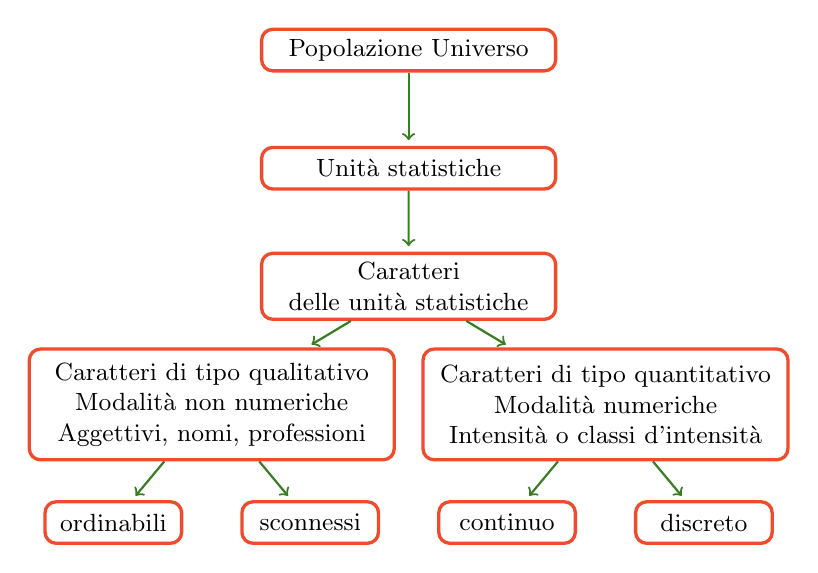
\begin{tikzpicture}[font=\small,
  punto/.style={%
    draw=RedOrange, 
    rectangle, 
    fill=white,
    very thick, 
    rounded corners,
    text centered,
    text width=35mm,
    minimum height=1.5em},
  subpunto/.style={%
    draw=RedOrange, 
    rectangle, 
    fill=white,
    very thick, 
    rounded corners,
    text centered,
    text width=44mm,
    minimum height=4em},
  subpunto1/.style={%
    draw=RedOrange, 
    rectangle, 
    fill=white,
    very thick, 
    rounded corners,
    text centered,
    text width=15mm,
    minimum height=1.5em},
  level distance=15mm,
  level 3/.style={sibling distance=50mm},
  level 4/.style={sibling distance=25mm}, 
  edge from parent/.style={draw,->,OliveGreen, thick, shorten >=2pt}]
  
\node [punto] {Popolazione Universo}
  child {node [punto] {Unit\`a statistiche}
    child {node [punto]{Caratteri \\delle unit\`a statistiche}
      child{node [subpunto]{Caratteri di tipo qualitativo \\Modalit\`a non numeriche \\Aggettivi, nomi, professioni}
	child {node [subpunto1]{ordinabili}}
	child {node [subpunto1]{sconnessi}}}
      child {node [subpunto]{Caratteri di tipo quantitativo \\Modalit\`a numeriche \\Intensit\`a o classi d'intensit\`a}
	child {node[subpunto1] {continuo}}
	child {node[subpunto1] {discreto}}}}};
\end{tikzpicture}

\end{center}

\ovalbox{\risolvii \ref{ese:A.2}, \ref{ese:A.3}, \ref{ese:A.5}, \ref{ese:A.6}, \ref{ese:A.7}, \ref{ese:A.8}, \ref{ese:A.9}}

\subsection{Rappresentazione grafica}

La rappresentazione grafica dei dati statistici facilita notevolmente lo studio delle caratteristiche del
fenomeno che si sta esaminando; infatti dopo aver impostato l'indagine, raccolto, classificato ed elaborato i dati nelle tabelle,
i dati non sempre si presentano in una forma di facile lettura ed il loro significato e la loro interpretazione rimane poco chiara.
Attraverso la rappresentazione grafica, i risultati dell'indagine emergono immediatamente, in maniera diretta e sintetica.

La rappresentazione grafica può avvenire utilizzando diversi tipi di grafico a seconda delle caratteristiche da
analizzare.

\subsubsection{Diagramma cartesiano}
La rappresentazione grafica attraverso un diagramma cartesiano dà, in modo immediato, informazioni sull'andamento globale del fenomeno e viene
utilizzata prevalentemente per la rappresentazione di serie storiche (per esempio, per rappresentare il numero di auto prodotte per anno da una fabbrica)
oppure quando si hanno due caratteri quantitativi e si vuol analizzare il tipo di legame esistente fra di essi.


\begin{exrig}
 \begin{esempio}

Consideriamo la tabella statistica relativa alla domanda ``quante ore al giorno passi al computer?'', posta ad un
campione di~50 ragazzi dai~16 ai~24 anni.

Rappresentiamo la tabella attraverso un diagramma cartesiano costruito tracciando due rette perpendicolari, gli assi, quello verticale orientato verso
l'alto e quello orizzontale orientato verso destra. Riportiamo sull'asse orizzontale il numero di ore e sull'asse verticale il numero di ragazzi e determiniamo
i punti aventi come coordinate (numero ore; numero ragazzi).

Il punto~$A$ avrà come coordinate~$(0;4)$, il punto~$B$ avrà come coordinate~$(1;6)$ e così via. Uniamo poi
i punti con segmenti e otteniamo il diagramma cartesiano~(grafico~\ref{gr:A.1}).
Precisamente~$A(0;4)$, $B(1;6)$, $C(2;12)$, $D(3;16)$, $E(4;8)$, $F(5;4)$, $G(6;2)$.

\begin{center}
\begin{tabular}{lccccccc}
\toprule
Numero di ore & 0 & 1 &2 & 3 & 4 & 5 & 6\\
Numero di ragazzi & 4 & 6 & 12 & 16 & 8 & 4 & 2 \\
\bottomrule
\end{tabular}
\end{center}
Dal grafico~\ref{gr:A.2} si può notare immediatamente che la maggior parte dei ragazzi trascorre dalle~2 alle~3 ore al computer dato che il picco più
alto si ha proprio nei punti~$C$ e~$D$.
Si può anche notare che, ad esempio, il punto~$X$ di coordinate~$(\np{3,5};12)$, appartenente al segmento di congiunzione tra i punti~$D$ ed~$E$,
non ha significato reale, dato che le sue coordinate non sono riportate nella tabella statistica del fenomeno da studiare.
\begin{grafico}[t]
\begin{minipage}{0.5\textwidth}
% (c) 2012 Dimitrios Vrettos - d.vrettos@gmail.com
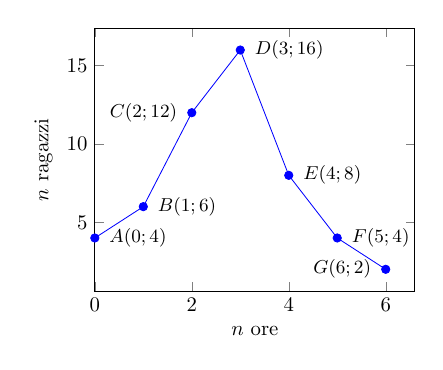
\begin{tikzpicture}[scale=.75]
  \tikzset{
    every pin/.style={pin distance=0,font=\small},
  }

\begin{axis}[xlabel=$n\grado$ ore, ylabel=$n\grado$ ragazzi,xmin=0]
  \addplot[color=blue, mark=*]
    coordinates{
      (0,4) 
      (1,6)
      (2,12)
      (3,16)
      (4,8)
      (5,4)
      (6,2)
      };

  \node[pin=0:{$A(0;4)$}] at (axis cs:0,4) {};
  \node[pin=0:{$B(1;6)$}] at (axis cs:1,6) {};
  \node[pin=180:{$C(2;12)$}] at (axis cs:2,12) {};
  \node[pin=0:{$D(3;16)$}] at (axis cs:3,16) {};
  \node[pin=0:{$E(4;8)$}] at (axis cs:4,8) {};
  \node[pin=0:{$F(5;4)$}] at (axis cs:5,4) {};
   \node[pin=180:{$G(6;2)$}] at (axis cs:6,2) {};
\end {axis}
\end{tikzpicture}

\caption{Esempio~24.4}\label{gr:A.1}
\end{minipage}\hfill
\begin{minipage}{0.5\textwidth}
% (c) 2012 Dimitrios Vrettos - d.vrettos@gmail.com
\begin{tikzpicture}[scale=.75]
  \tikzset{
    every pin/.style={pin distance=0,font=\small},
  }

  \begin{axis}[xlabel=$n\grado$ ore, ylabel=$n\grado$ ragazzi,xmin=0]
    \addplot[only marks, color=blue, mark=*]
      coordinates{
	(0,4) 
	(1,6)
	(2,12)
	(5,4)
	(6,2)
      };
 \addplot[color=grigio70, mark=*]
      coordinates{
	(0,4)
	(1,6)
	(2,12)
   (3,16)
      };    
 \addplot[color=grigio70, mark=*]
      coordinates{
	(6,2)
	(5,4)
	(4,8)
      };
 \addplot[color=blue, mark=*]
      coordinates{
	(3,16)
	(4,8)
      };
 \addplot[color=red, mark=*]
      coordinates{
	(3.5,12)
      };

    \node[pin=0:{$A(0;4)$}] at (axis cs:0,4) {};
    \node[pin=0:{$B(1;6)$}] at (axis cs:1,6) {};
    \node[pin=180:{$C(2;12)$}] at (axis cs:2,12) {};
    \node[pin=0:{$D(3;16)$}] at (axis cs:3,16) {};
    \node[pin=0:{$E(4;8)$}] at (axis cs:4,8) {};
    \node[pin=0:{$F(5;4)$}] at (axis cs:5,4) {};
    \node[pin=180:{$G(6;2)$}] at (axis cs:6,2) {};
    \node[pin=0:{$X(3,5;12)$}] at (axis cs:3.5,12) {};
  \end {axis}
\end{tikzpicture}

\caption{Esempio~24.4}\label{gr:A.2}
\end{minipage}
\end{grafico}
\end{esempio}
\end{exrig}

\subsubsection{Ideogramma}
Nella rappresentazione grafica attraverso \emph{ideogramma} si rappresenta un certo numero di dati con un simbolo che si assume come \emph{unità grafica};
il simbolo deve richiamare l'oggetto dell'indagine e dare quindi una visione immediata del fenomeno.
Ad esempio si può utilizzare un uomo stilizzato per rappresentare un dato riguardante il numero di persone che vivono in un determinato territorio,
una macchina per la produzione annua di automobili in una fabbrica, e così via.
Tale tipo di rappresentazione è spesso usata in campo pubblicitario perché caratterizzata da un evidente impatto visivo.

\begin{exrig}
 \begin{esempio}

Un istituto scolastico ha visto aumentare i suoi iscritti, dall'anno scolastico~2003-2004 all'anno~2008-2009 secondo quanto riportato nella seguente tabella:

\begin{center}
 \begin{tabular}{lcccccc}
 \toprule
 Anno scolastico & 2003-04 & 2004-05 & 2005-06 & 2006-07 & 2007-08 & 2008-09\\
 Iscritti & 150 & 200 & 200 & 325 & 375 & 450\\
 \bottomrule
\end{tabular}
\end{center}

Possiamo rappresentare mediante ideogramma i dati contenuti nella tabella statistica.
Consideriamo una faccina stilizzata come unità grafica assegnandole il valore di~50 ragazzi iscritti.
\begin{center}
 % (c) 2012 Dimitrios Vrettos - d.vrettos@gmail.com

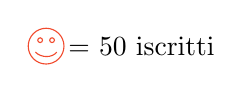
\begin{tikzpicture}
\begin{scope}[RedOrange]
\draw(0,-.5ex) circle (1.5ex);
\foreach \x in {-.5ex,.5ex}
  \draw[fill=white] (\x,0) circle (.2ex);
   \draw (-.9ex,-1ex)..controls (-0.4ex,-1.5ex)and(0.5ex,-1.5ex)..(.9ex,-1ex);
\end{scope}
\node () at (8ex,-.5ex) { $=$ 50 iscritti};
\end{tikzpicture}

\end{center}
Il numero degli iscritti di ogni anno scolastico sarà rappresentato da tante unità grafiche quanti sono i gruppi di~50 iscritti.
Per avere il grafico relativo all'anno~2003-2004 si devono usare tre faccine, in quanto~$150:50=3$.
\begin{center}
 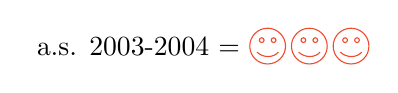
\begin{tikzpicture}
\begin{scope}[RedOrange]
\foreach \xi in {0,3.5ex,7ex}{
\draw(\xi,-.5ex) circle (1.5ex);
   \draw (\xi-.9ex,-1ex)..controls (\xi-0.4ex,-1.5ex)and(\xi+0.5ex,-1.5ex)..(\xi+.9ex,-1ex);}
\foreach \xii in {-.5ex,.5ex,3ex,4ex,6.5ex,7.5ex}
  \draw[fill=white] (\xii,0) circle (.2ex);
\end{scope}
\node[left] at (-1.5ex,-.5ex) { a.s. 2003-2004 $=$};
\end{tikzpicture}

\end{center}
Se la divisione del numero degli iscritti per~50 dà resto, esso si dovrà rappresentare disegnando solo una parte
dell'unità grafica, corrispondente alla frazione tra resto e~50. Ad esempio nell'~a.s.~2006-2007 ci sono stati~325 iscritti; $325:50 = 6$
col resto di~25, quindi~325 sarà uguale a~6 unità grafiche e~$\frac{25}{50}=\frac{1}{2}$ unità grafica, cioè mezza faccina, ovvero $325:50 = \np{6,5}$ cioè 6 faccine e mezzo.
\begin{center}
 % (c) 2012 Dimitrios Vrettos - d.vrettos@gmail.com

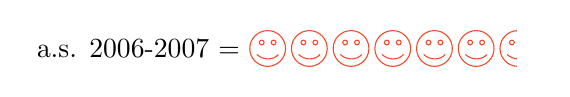
\begin{tikzpicture}
\begin{scope}[RedOrange]
\foreach \xi in {0,3.5ex,7ex,10.5ex,14ex,17.5ex,21ex}{
\draw(\xi,-.5ex) circle (1.5ex);
   \draw (\xi-.9ex,-1ex)..controls (\xi-0.4ex,-1.5ex)and(\xi+0.5ex,-1.5ex)..(\xi+.9ex,-1ex);}
\foreach \xii in {-.5ex,.5ex,3ex,4ex,6.5ex,7.5ex,10ex,11ex,13.5ex,14.5ex,17ex,18ex,20.5ex,21.5ex}
  \draw[fill=white] (\xii,0) circle (.2ex);
\end{scope}
\filldraw[white] (21ex,-2.2ex) rectangle (23ex,1.2ex);
\node[left] at (-1.5ex,-.5ex) { a.s. 2006-2007 $=$};
\end{tikzpicture}

\end{center}

Il grafico completo sarà:
\begin{center}
 % (c) 2012 Dimitrios Vrettos - d.vrettos@gmail.com

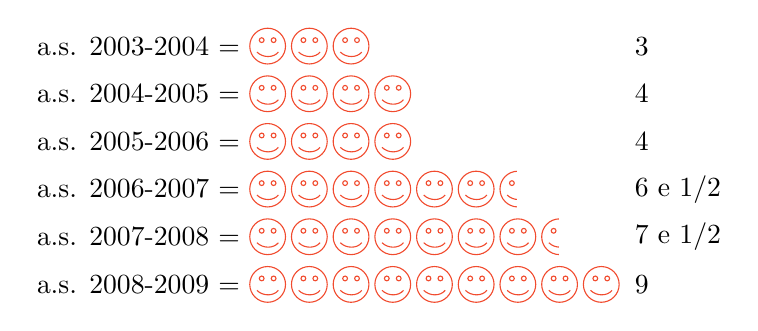
\begin{tikzpicture}[RedOrange]
  \foreach \xi in {0,3.5ex,7ex}{
    \draw(\xi,-.5ex) circle (1.5ex);
    \draw (\xi-.9ex,-1ex)..controls (\xi-0.4ex,-1.5ex)and(\xi+0.5ex,-1.5ex)..(\xi+.9ex,-1ex);
  }
  \foreach \xii in {-.5ex,.5ex,3ex,4ex,6.5ex,7.5ex}
    \draw[fill=white] (\xii,0) circle (.2ex);
  
  \node[left,black] at (-1.5ex,-.5ex) { a.s. 2003-2004 $=$};
  \node[right,black] at(30ex,-.5ex){3};

  \begin{scope}[yshift=-4ex]
    \foreach \xi in {0,3.5ex,7ex,10.5ex}{
      \draw(\xi,-.5ex) circle (1.5ex);
      \draw (\xi-.9ex,-1ex)..controls (\xi-0.4ex,-1.5ex)and(\xi+0.5ex,-1.5ex)..(\xi+.9ex,-1ex);
    }
    \foreach \xii in {-.5ex,.5ex,3ex,4ex,6.5ex,7.5ex,10ex,11ex}
      \draw[fill=white] (\xii,0) circle (.2ex);
    \node[left,black] at (-1.5ex,-.5ex) { a.s. 2004-2005 $=$};
    \node[right,black] at(30ex,-.5ex){4};
  \end{scope}

  \begin{scope}[yshift=-8ex]
    \foreach \xi in {0,3.5ex,7ex,10.5ex}{
      \draw(\xi,-.5ex) circle (1.5ex);
      \draw (\xi-.9ex,-1ex)..controls (\xi-0.4ex,-1.5ex)and(\xi+0.5ex,-1.5ex)..(\xi+.9ex,-1ex);}
    \foreach \xii in {-.5ex,.5ex,3ex,4ex,6.5ex,7.5ex,10ex,11ex}
      \draw[fill=white] (\xii,0) circle (.2ex);
    \node[left,black] at (-1.5ex,-.5ex) { a.s. 2005-2006 $=$};
    \node[right,black] at(30ex,-.5ex){4};
  \end{scope}

  \begin{scope}[yshift=-12ex]
    \foreach \xi in {0,3.5ex,7ex,10.5ex,14ex,17.5ex,21ex}{
      \draw(\xi,-.5ex) circle (1.5ex);
      \draw (\xi-.9ex,-1ex)..controls (\xi-0.4ex,-1.5ex)and(\xi+0.5ex,-1.5ex)..(\xi+.9ex,-1ex);}
    \foreach \xii in {-.5ex,.5ex,3ex,4ex,6.5ex,7.5ex,10ex,11ex,13.5ex,14.5ex,17ex,18ex,20.5ex,21.5ex}
      \draw[fill=white] (\xii,0) circle (.2ex);
    \node[left, black] at (-1.5ex,-.5ex) { a.s. 2006-2007 $=$};\filldraw[white] (21ex,-2.2ex) rectangle (23ex,1.2ex);
    \node[right,black] at(30ex,-.5ex){6 e  1/2};
  \end{scope}

  \begin{scope}[yshift=-16ex]
    \foreach \xi in {0,3.5ex,7ex,10.5ex,14ex,17.5ex,21ex,24.5ex}{
      \draw(\xi,-.5ex) circle (1.5ex);
      \draw (\xi-.9ex,-1ex)..controls (\xi-0.4ex,-1.5ex)and(\xi+0.5ex,-1.5ex)..(\xi+.9ex,-1ex);}
    \foreach \xii in {-.5ex,.5ex,3ex,4ex,6.5ex,7.5ex,10ex,11ex,13.5ex,14.5ex,17ex,18ex,20.5ex,21.5ex,24ex,25ex}
      \draw[fill=white] (\xii,0) circle (.2ex);
    \node[left, black] at (-1.5ex,-.5ex) { a.s. 2007-2008 $=$};\filldraw[white] (24.5ex,-2.2ex) rectangle (26.5ex,1.2ex);
    \node[right,black] at(30ex,-.5ex){7 e  1/2};
  \end{scope}

  \begin{scope}[yshift=-20ex]
    \foreach \xi in {0,3.5ex,7ex,10.5ex,14ex,17.5ex,21ex,24.5ex,28ex}{
      \draw(\xi,-.5ex) circle (1.5ex);
      \draw (\xi-.9ex,-1ex)..controls (\xi-0.4ex,-1.5ex)and(\xi+0.5ex,-1.5ex)..(\xi+.9ex,-1ex);}
    \foreach \xii in {-.5ex,.5ex,3ex,4ex,6.5ex,7.5ex,10ex,11ex,13.5ex,14.5ex,17ex,18ex,20.5ex,21.5ex,24ex,25ex,27.5ex,28.5ex}
      \draw[fill=white] (\xii,0) circle (.2ex);
    \node[left, black] at (-1.5ex,-.5ex) { a.s. 2008-2009 $=$};
    \node[right,black] at(30ex,-.5ex){9};
    \end{scope}
\end{tikzpicture}

\end{center}
 \end{esempio}
\end{exrig}

\subsubsection{Diagramma a barre o a colonne}

Questo tipo di rappresentazione, detta anche diagramma a nastri o a bastoni, viene usata quando si vuole fornire un'idea delle frequenze
delle diverse modalità di un fenomeno. In genere si usa per caratteri qualitativi o quantitativi discreti.
Per poter valutare il significato statistico della lunghezza delle barre (o delle colonne) è necessario scegliere opportunamente una scala di riferimento:
la larghezza della barra (o della colonna) è arbitraria ma uguale per tutte le barre (o colonne) e la sua lunghezza è proporzionale alla caratteristica che si deve rappresentare.
Le barre (o le colonne) possono inoltre essere suddivise in parti di colori diversi per indicare le singole componenti o i singoli fenomeni
che si vogliono analizzare.

La differenza fra la rappresentazione a barre e quella a colonne consiste soltanto
nell'orientamento del grafico: nel diagramma a barre si indicano le modalità del carattere sull'asse verticale e le frequenze sull'asse orizzontale,
mentre in quello a colonne le modalità del carattere sono riportate sull'asse
orizzontale e le frequenze su quello verticale.

Di seguito vengono riportate le due tipologie di grafico accompagnate dalla tabella di riferimento:
\begin{center}
 \begin{tabularx}{.95\textwidth}{X*{7}{c}Xc}
\toprule
Materia& Italiano &Storia & Geografia & Matem. & Scienze & Ed. Fisica & Totale\\
Maschi & 5 & 4& 4 & 2& 6 & 5& 26\\
Femmine & 3 & 7 & 2 & 3  & 4 & 5 & 24\\
\bottomrule
\end{tabularx}
\end{center}

\begin{center}
\begin{figure}[!ht]
% (c) 2012 Dimitrios Vrettos - d.vrettos@gmail.com

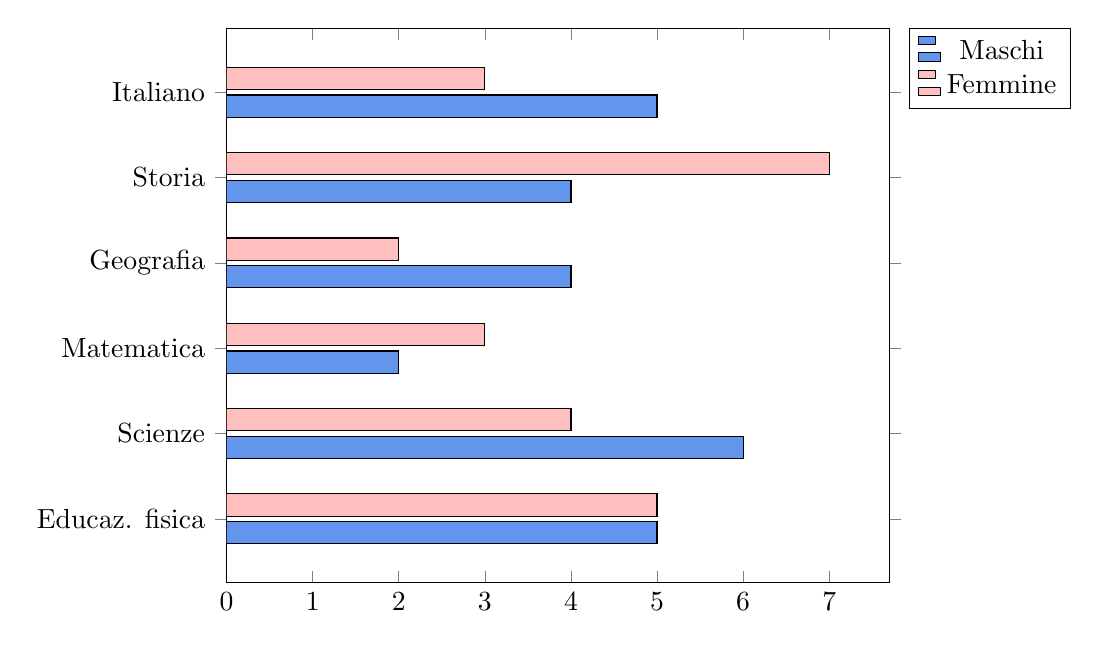
\begin{tikzpicture}
\begin{axis}[
legend entries={Maschi, Femmine},
legend pos=outer north east,
xbar,
enlarge y limits=0.15,
symbolic y coords={Educaz. fisica,Scienze,Matematica, Geografia,Storia,Italiano },
ytick=data,
bar width=8pt, 
xmin=0, 
width=100mm]

\addplot[fill=CornflowerBlue, draw=black] coordinates {
(5,Educaz. fisica)
(6,Scienze)
(2,Matematica)
(4,Geografia)
(4,Storia)
(5,Italiano)
};

\addplot[fill=pink, draw=black] coordinates{
(5,Educaz. fisica)
(4,Scienze)
(3,Matematica)
(2,Geografia)
(7,Storia)
(3,Italiano)
};
\end{axis}
\end{tikzpicture}

\caption{Diagramma a barre}
\end{figure}
\end{center}

\begin{center}
 \begin{figure}[!ht]
% (c) 2012 Dimitrios Vrettos - d.vrettos@gmail.com

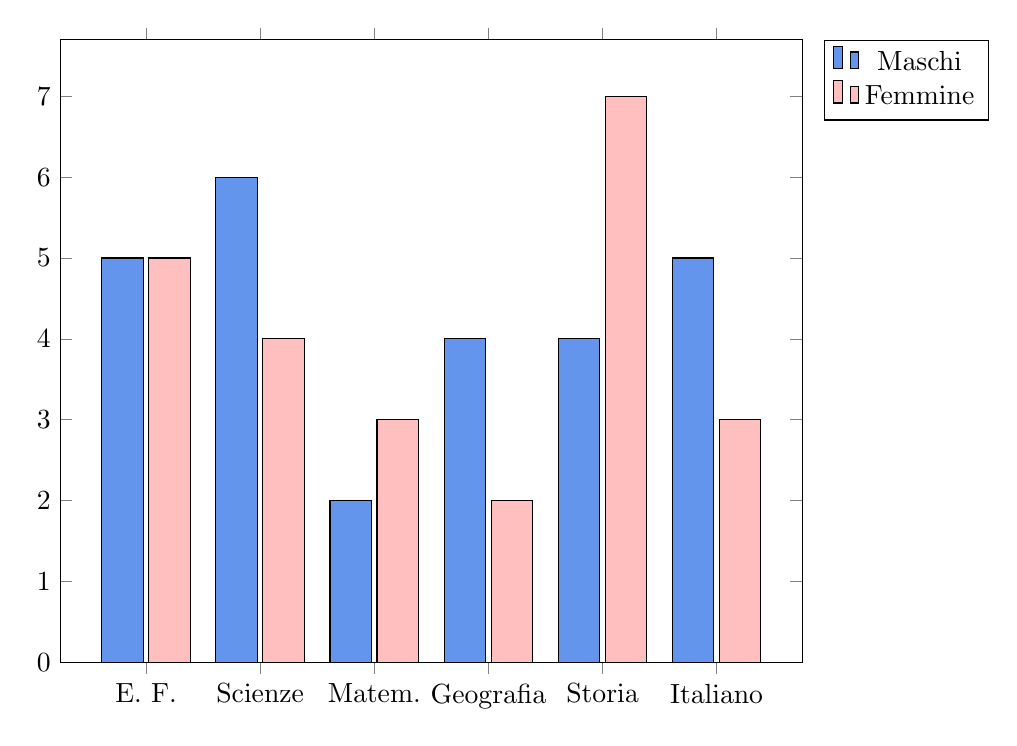
\begin{tikzpicture}
\begin{axis}[
legend entries={Maschi, Femmine},
legend pos=outer north east,
ybar,
enlarge x limits=0.15,
symbolic x coords={E. F.,Scienze,Matem., Geografia,Storia,Italiano },
xtick=data,
bar width=15pt, 
ymin=0, 
width=110mm]

\addplot[fill=CornflowerBlue, draw=black] coordinates {
(E. F.,5)
(Scienze,6)
(Matem.,2)
(Geografia,4)
(Storia,4)
(Italiano,5)
};
 
 \addplot[fill=pink, draw=black] coordinates{
 (E. F.,5)
 (Scienze,4)
 (Matem.,3)
 (Geografia,2)
 (Storia,7)
 (Italiano,3)
 };
\end{axis}
\end{tikzpicture}

\caption{Diagramma a colonne}
\end{figure}
\end{center}

\subsubsection{Areogramma}

Questo tipo di rappresentazione, detta anche grafico a torta, viene utilizzato quando si vogliono evidenziare le parti che compongono un fenomeno, per esempio per indicare
come si dividono gli alunni di una classe in maschi e femmine, o per rappresentare in che modo
le varie voci di spesa incidono sul bilancio familiare.
Il grafico si ottiene dividendo un cerchio in settori circolari con aree direttamente proporzionali alle frequenze che rappresentano.
Per disegnare l'areogramma, si disegna una circonferenza di diametro arbitrario e si fa corrispondere l'angolo al centro di~$360\grado$,
con il~$100\%$ di frequenza percentuale; per ottenere l'angolo corrispondente ad una certa frequenza percentuale $f_x$ si risolve la proporzione~$360\grado:X\grado=100:f_x\:\Rightarrow\:X\grado = \np{3,6} \cdot f_x$.
Si suddivide così la circonferenza negli angoli ottenuti e si evidenziano in maniera differente tra loro i settori circolari ottenuti.

\begin{exrig}
 \begin{esempio}
Consideriamo la seguente tabella statistica che indica gli studenti di un dato istituto scolastico divisi per classe frequentata, in un dato anno.

\begin{center}
\begin{tabular}{lcccccc}
\toprule
Classe & 1\textsuperscript{a} &2\textsuperscript{a} &3\textsuperscript{a} & 4\textsuperscript{a} &5\textsuperscript{a} &Totale\\
Studenti & 320 & 230 & 212 & 152 & 96 & $\np{1010}$ \\
\bottomrule
\end{tabular}
\end{center}

Nella tabella sono indicate le frequenze assolute; calcoliamo ora le frequenze percentuali degli studenti.
Per la~1\textsuperscript{a} classe si ha:~$\frac{320}{\np{1010}}=\np{0,32}$ arrotondato alla seconda cifra decimale, che equivale al~$32\%$ e così via per le classi successive.

\begin{center}
\begin{tabular}{lcccccc}
\toprule
Classe & 1\textsuperscript{a} & 2\textsuperscript{a} & 3\textsuperscript{a} & 4\textsuperscript{a} & 5\textsuperscript{a} & Totale \\
 Frequenze percentuali& $32\%$ & $23\%$ & $21\%$ & $15\%$ & $9\%$ & $100\%$ \\
\bottomrule
\end{tabular}
\end{center}

Rappresentiamo graficamente mediante areogramma i dati contenuti nella tabella precedente.
\begin{center}
 \begin{tikzpicture}[x=10mm,y=10mm, x radius=10mm, y radius=10mm]
  \draw (0,0) circle (3);
  \draw[pattern=north east lines,pattern color=orange] (0,0) -- (0:3) arc (0:115.2:3);
  \draw[pattern=horizontal lines,pattern color=brown] (0,0)-- (115.2:3) arc (115.2:198:3);
  \draw[pattern=dots,pattern color=green] (0,0)-- (198:3) arc (198:273.6:3);
  \draw[pattern=north west lines,pattern color=red] (0,0)-- (273.6:3) arc (273.6:327.6:3);
  \draw[pattern=vertical lines,pattern color=blue] (0,0)-- (327.6:3) arc (327.6:360:3);

  \begin{scope}[every node/.style={rounded corners, draw=black, fill=white}]
    \draw(57.6:2) node {$115,2\grado $};
    \draw(156.6:2) node {$82,8\grado $};
    \draw(235.8:2) node {$75,6\grado $};
    \draw(300.6:2) node {$54\grado $};
    \draw(343.8:2) node {$32,4\grado $};
  \end{scope}

  \begin{scope}[thin, <->]
    \draw (0:1) arc (0:115.2:1);
    \draw (115.2:.8) arc (115.2:198:.8);
    \draw (198:1.2) arc (198:273.6:1.2);
    \draw (273.6:.8) arc (273.6:327.6:.8);
    \draw (327.6:1.1) arc (327.6:360:1.1);
  \end{scope}

  \draw(57.6:4) node {1\textsuperscript{a} classe: $32\%$};
  \draw[left](156.3:3) node {2\textsuperscript{a} classe: $23\%$};
  \draw(235.8:4) node {3\textsuperscript{a} classe: $21\%$};
  \draw[below right](300.6:3) node {4\textsuperscript{a} classe: $15\%$};
  \draw[right](343.8:3) node {5\textsuperscript{a} classe: $9\%$};
\end{tikzpicture}

\end{center}

Per ottenere l'angolo relativo alla frequenza percentuale della~1\textsuperscript{a} classe si fa:~$\np{3,6} \cdot 32=\np{115,2}\grado$ e
per la~2\textsuperscript{a} classe:~$\np{3,6} \cdot 23=\np{82,2}\grado$ e così via per le altre classi.

Dal grafico si può notare immediatamente che la classe più frequentata è la prima.

 \end{esempio}
\end{exrig}

\subsubsection{Istogramma}

Si utilizza la rappresentazione grafica attraverso istogramma quando il carattere analizzato è di tipo quantitativo ed i dati sono raggruppati in classi.

Prima di tutto si distribuiscono i dati in classi o gruppi e si determina il numero di unità appartenenti a ciascuna classe; questo numero è
detto \emph{frequenza della classe}.
Riportando tali dati in una tabella si ottiene la distribuzione delle frequenze. Poiché le classi potrebbero avere ampiezze diverse si calcola
la \emph{densità di frequenza}, definita come il rapporto fra la frequenza della classe e la relativa ampiezza.

Per disegnare un istogramma si tracciano due assi; sull'asse verticale, orientato verso l'alto, si fissa un segmento unitario e vi si riportano
le densità di frequenza. L'asse orizzontale, orientato verso destra, è invece suddiviso in tanti segmenti la cui ampiezza è pari a quella delle singole classi.
Il grafico consiste in un insieme di rettangoli aventi per base ogni classe e altezza la densità di frequenza corrispondente.
In tal modo l'area di ogni rettangolo rappresenta la frequenza corrispondente a ciascuna classe.

\begin{exrig}
 \begin{esempio}

Costruiamo un istogramma a partire dalla distribuzione di frequenza riportata nella seguente tabella:
\begin{center}
\begin{tabular}{cc}
\toprule
Diametro crateri lunari ($\unit{km}$) & Numero di crateri\\
\midrule
$0-50$ & $\np{1088}$ \\
$50-100$ & $745$ \\
$100-150$ & $20$ \\
\bottomrule
\end{tabular}
\end{center}

Innanzi tutto per ogni classe dobbiamo determinare la densità di frequenza, che si ottiene dividendo la frequenza assoluta per l'ampiezza della classe:

\begin{center}
\begin{tabular}{cc}
\toprule
Diametro crateri lunari ($\unit{km}$) & Densità di freq.\\
\midrule
$0-50$ & $\np{1088}/50=\np{21,76}$ \\
$50-100$ & $745/50=\np{14,9}$ \\
$100-150$ & $20/50=\np{0,4}$ \\
\bottomrule
\end{tabular}
\end{center}

\begin{center}
% (c) 2012 Dimitrios Vrettos - d.vrettos@gmail.com

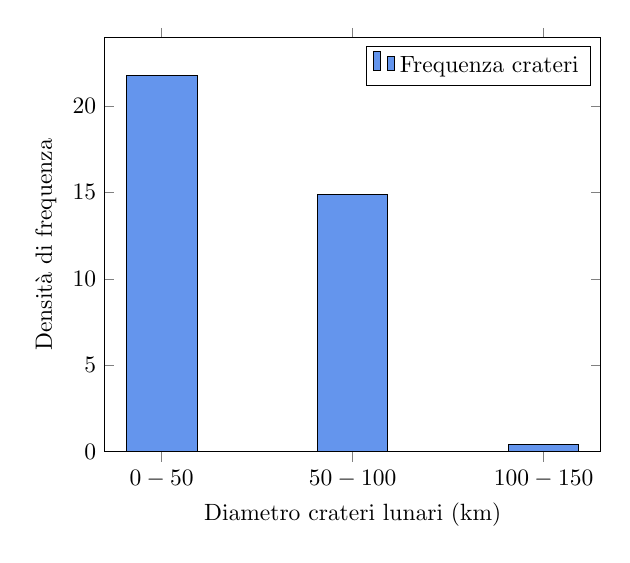
\begin{tikzpicture}[scale=.85]
\begin{axis}[
xlabel=Diametro crateri lunari (km), ylabel=Densità di frequenza,
legend entries={Frequenza crateri},
ybar,
enlarge x limits=0.15,
symbolic x coords={$0-50$,$50-100$,$100-150$},
xtick=data,
bar width=30pt, 
ymin=0, 
width=90mm]

\addplot[fill=CornflowerBlue, draw=black] coordinates {
($0-50$,21.76)
($50-100$,14.9)
($100-150$,.4)
 };
 
\end{axis}
\end{tikzpicture}

\end{center}
\end{esempio}

\begin{esempio}
Consideriamo la seguente tabella statistica che riporta i giorni di pioggia di ogni mese, in un dato anno e in una data città.

\begin{center}
\begin{tabular}{lclc}
\toprule
Mesi & Giorni di pioggia &Mesi & Giorni di pioggia\\
\midrule
Gennaio & 15&Luglio & 1 \\
Febbraio & 10 &Agosto & 3\\
Marzo & 14 &Settembre & 3\\
Aprile & 8 &Ottobre & 5\\
Maggio & 5 &Novembre & 9\\
Giugno & 2 &Dicembre & 11\\
\bottomrule
\end{tabular}
\end{center}
Dividiamo i mesi dell'anno in classi, raggruppandoli in stagioni. Ad esempio, Luglio, Agosto e Settembre
appartengono alla classe dell'Estate e la frequenza di questa classe è data dalla somma delle frequenze di ogni mese, cioè~$1 + 3 + 3 = 7$. Si prosegue in questo modo per ogni classe ottenendo così la distribuzione delle frequenze riportata nella tabella.
\begin{center}
\begin{tabular}{lcccc}
\toprule
Stagioni & Estate & Autunno & Inverno& Primavera\\
Giorni di pioggia & 7 & 25 & 39 & 15 \\
\bottomrule
\end{tabular}
\end{center}
Costruisci ora l'istogramma corrispondente alla tabella precedente riportando sull'asse orizzontale le classi (stagioni) e su quello verticale le densità di frequenze.
 \end{esempio}
\end{exrig}

\ovalbox{\risolvii \ref{ese:A.10}, \ref{ese:A.11}, \ref{ese:A.12}, \ref{ese:A.13}, \ref{ese:A.14}, \ref{ese:A.15}, \ref{ese:A.16}, \ref{ese:A.17}, \ref{ese:A.18}, \ref{ese:A.19}, \ref{ese:A.20}}

\section{Indici di posizione}

Nel caso in cui il carattere considerato nell'indagine sia di tipo quantitativo, l'andamento dei dati raccolti può essere sinteticamente descritto per mezzo di opportuni indici. Gli \emph{indici di posizione} vengono utilizzati per dare un'indicazione sulla distribuzione delle frequenze per mezzo di un solo numero.
A seconda del carattere oggetto dell'indagine statistica possono essere utilizzati indici differenti.

\subsection{Moda}

\begin{definizione}
La \emph{moda} è la modalità del carattere indagato che si presenta più frequentemente.
\end{definizione}

In una successione di~$n$ modalità~$x_1$, $x_2$, \ldots, $x_n$
con le relative frequenze~$f_1$, $f_2$, \ldots, $f_n$, la moda è la modalità che ha la frequenza maggiore.
Questo valore può essere calcolato per qualunque tipo di carattere, sia qualitativo che quantitativo.
Se il carattere è quantitativo continuo con dati raggruppati in classi non è possibile determinare con esattezza la moda, ci si limita
ad individuare la \emph{classe modale} definita come la classe cui è associata la massima densità di frequenza.

\begin{exrig}
 \begin{esempio}

 Nella tabella seguente sono riportati i numeri degli studenti, divisi per classe, della sezione~A di un dato istituto,
 in un dato anno. Si può osservare che la~1\textsuperscript{a} classe presenta la frequenza massima di~320 studenti, quindi la moda è la classe prima.
\begin{center}
\begin{tabular}{lcccccc}
\toprule
Classe & 1$\grado$ & 2$\grado$ & 3$\grado$ & 4$\grado$ & 5$\grado$ & Totale \\
Studenti & 320 & 230 & 212 & 152 & 96 & 1\,010 \\
\bottomrule
\end{tabular}
\end{center}
 \end{esempio}

\begin{esempio}
La tabella raccoglie i dati relativi alla domanda ``quante ore alla settimana pratichi sport?'', posta ad un
campione di~50 ragazzi dai~18 ai~25 anni. Si può osservare che~12 e~18 ore presentano la frequenza massima~14, quindi si hanno due
mode~12 ore e~18 ore. In questo caso la distribuzione è bimodale.


\begin{center}
\begin{tabular}{lcccccccc}
\toprule
Numero di ore & 0 &4 &8 &12 &16 &18 &22 &Totale\\
 Numero di ragazzi& 4 & 1 & 3 & 14 & 8 & 14 & 6 & 50 \\
\bottomrule
\end{tabular}
\end{center}
 \end{esempio}

 \begin{esempio}
La tabella seguente è relativa alla distribuzione delle classi di altezza di un gruppo di studenti.

\begin{center}
\begin{tabular}{lcccccc}
\toprule
Altezza (cm) &160-165 &165-170 &170-175 &175-185 &185-200 &Totale \\
Numero di studenti & 5 & 8 & 15 & 10 & 2 & 40 \\
\bottomrule
\end{tabular}
\end{center}
Poiché le classi hanno ampiezza diversa è necessario calcolare la densità di frequenza.

\begin{center}
\begin{tabular}{lccccc}
\toprule
Altezza &160-165 &165-170 &170-175 &175-185 &185-200 \\
Densità di frequenza & 1 & $\np{1,6}$ & 3 & 1 & $\np{0,13}$ \\
\bottomrule
\end{tabular}
\end{center}
La massima densità di frequenza si ha in corrispondenza della classe~170-175, essa rappresenta quindi la classe modale.
 \end{esempio}
\end{exrig}

\subsection{Media aritmetica}

\begin{definizione}
La \emph{media aritmetica} (semplice) è il valore ottenuto sommando tutti i dati e
dividendo tale somma per il numero dei dati.
\end{definizione}

Se abbiamo~$n$ dati~$x_1$, $x_2$, \ldots, $x_n$, la media aritmetica semplice~$M$ è data da:

\begin{equation*}
M=\frac{x_1+x_2+ \dots +x_n}{n}=\frac{1}{n}\sum_{i=1}^n x_i.
\end{equation*}

\begin{exrig}
 \begin{esempio}

Riprendiamo in esame la tabella relativa agli studenti, divisi per classe frequentata di un dato istituto scolastico, in un dato anno e calcoliamone la media aritmetica semplice.
\begin{center}
 \begin{tabular}{lcccccc}
 \toprule
 Classe & 1\textsuperscript{a} & 2\textsuperscript{a} & 3\textsuperscript{a} & 4\textsuperscript{a} & 5\textsuperscript{a} & Totale\\
 Studenti & 320 & 230 & 212 & 152 & 96 & $\np{1010}$\\
 \bottomrule
\end{tabular}
\end{center}
Per calcolare la media aritmetica semplice degli studenti, sommiamo tutti gli studenti delle cinque classi e dividiamo tale somma per il numero delle classi:
\begin{equation*}
M=\frac{320+230+212+152+96}{5}= \frac{\np{1010}}{5}= 202.
\end{equation*}
Possiamo dire che si hanno mediamente~202 studenti per ogni classe.

\begin{definizione}
Si definisce \emph{scarto dalla media} (aritmetica) la differenza tra i valori osservati e la media.
\end{definizione}

Se~$x_1$, $x_2$, \ldots, $x_n$ sono i valori osservati e $M$ la loro media aritmetica, gli scarti sono~$s_1=x_1-M$, $s_2=x_2-M$, \ldots, $s_n=x_n-M$.
\end{esempio}

\begin{esempio}
Calcoliamo gli scarti dalla media per la distribuzione ``studenti per tipologia di classe frequentata'', la cui media è~$\np{1010}/5 = 202$.
\begin{center}
\begin{tabular}{l*{6}{c}}
\toprule
Classe & 1\textsuperscript{a} & 2\textsuperscript{a} & 3\textsuperscript{a} & 4\textsuperscript{a} & 5\textsuperscript{a} & Totale\\
Studenti & 320& 230& 212& 152& 96& $\np{1010}$ \\
Scarto & 118 & 28 & 10 & $-50$ & 106 & 0\\
\bottomrule
\end{tabular}
\end{center}
Si può osservare che vi solo valori superiori alla media e altri inferiori, tanto che lo scarto è rappresentato in
alcuni casi da un numero positivo, in altri da un numero negativo. Si può verificare che la somma degli scarti dalla media è nulla,
cioè gli scarti positivi compensano sempre quelli negativi.
 \end{esempio}
\end{exrig}


\begin{definizione}
La \emph{media aritmetica ponderata} è il valore ottenuto moltiplicando ciascuna modalità del carattere
dato con la propria frequenza, sommando tutti i prodotti fra loro e dividendo poi per la somma delle frequenze
(che equivale al numero totale $n$ delle unità statistiche considerate).
\end{definizione}

La media aritmetica ponderata si usa nel caso in cui le unità statistiche sono molte ed è già stata fatta la tabella delle frequenze. Avendo quindi le modalità del carattere~$m_1$, $m_2$, \ldots, $m_k$ e le relative frequenze~$f_1$, $f_2$, \ldots, $f_k$, la media aritmetica ponderata~$M$ è data da:
\begin{equation*}
M=\frac{m_1\cdot f_1+m_2\cdot f_2+ \dots +m_k\cdot f_k}{f_1+f_2+ \dots +f_k}=\frac{\sum_{i=1}^k m_i\cdot f_i}{\sum_{i=1}^k f_i}=\frac{1}{n}\sum_{i=1}^k m_i\cdot f_i.
\end{equation*}

\begin{exrig}
 \begin{esempio}

Riprendiamo la tabella dell'esempio precedente relativa alla domanda ``quante ore al giorno passi al computer?'',
posta ad un campione di~52 ragazzi dai~16 ai~24 anni. Calcoliamo la media aritmetica ponderata.
\begin{center}
 \begin{tabular}{lcccccccc}
 \toprule
 Numero di ore & 0 & 1 & 2 & 3 & 4 & 5 & 6 & Totale\\
 Numero di ragazzi & 4 & 6 & 12 & 16 & 8 & 4 & 2 & 52\\
 \bottomrule
\end{tabular}
\end{center}

Considerando le~7 modalità del carattere ``Numero di ore'' riportate nella tabella, si ha:
\begin{equation*}
M=\frac{0\cdot 4+1\cdot 6+2\cdot 12+3\cdot 16+4\cdot 8+5\cdot 4+6\cdot 2}{4+6+12+16+8+4+2}=\frac{142}{52}=\np{2,73}.
\end{equation*}

Possiamo dire che, in media, ciascun ragazzo passa circa~3 ore al giorno al computer.
\end{esempio}
\end{exrig}

Il valore della media aritmetica semplice effettuata sulle singole unità statistiche coincide con quella ponderata effettuata sul raggruppamento dei dati per modalità del carattere considerato (tabella delle frequenze).

\subsection{Mediana}
\begin{definizione}
La \emph{mediana} di una successione di dati disposti in ordine crescente è il valore equidistante dagli estremi, cioè è
\begin{itemize}
\item il dato che occupa la posizione centrale, se il numero dei dati è dispari;
\item è la media aritmetica dei dati della coppia centrale, se il numero dei dati è pari.
\end{itemize}
\end{definizione}

Poiché per calcolare la mediana i dati devono essere ordinati, è bene sottolineare che tale indice non può essere calcolato se il carattere in esame è di tipo qualitativo non ordinabile.

\begin{exrig}
\begin{esempio}
Supponiamo di avere~7 dati disposti in ordine crescente: 5, 8, 10, 14, 18, 20, 25.
Allora la mediana è il valore centrale, quello che occupa la quarta posizione, cioè il~14.
\end{esempio}

\begin{esempio}
Supponiamo di avere~8 dati disposti in ordine crescente: 1, 5, 8, 10, 14, 18, 20, 25.
La mediana è la media aritmetica dei dati che occupano la~4\textsuperscript{a} e la~5\textsuperscript{a} posizione, cioè~$\frac{10+14}{2}=12$.
\end{esempio}

\begin{esempio}
Supponiamo di avere la distribuzione di frequenza riportata nella tabella.
Il numero di osservazioni è pari, quindi la mediana è il valore della variabile che corrisponde alla media dei due
valori centrali, rispettivamente quelli che nella serie ordinata occupano il~13$\grado$ e il~14$\grado$ posto.

È necessario in questo caso determinare le \emph{frequenze cumulate}. Esse si ottengono sommando le frequenze che hanno un valore della
variabile minore o uguale alla modalità considerata.
La frequenza cumulata relativa al voto~3 rimane~2, quella relativa al voto~4 si ottiene sommando
la frequenza del~3 e la frequenza del~4, cioè~$2+2=4$, la frequenza cumulata relativa al voto~5 si ottiene dalla somma
della frequenza del~3, del~4 e del~5 e così via. Il~14$\grado$ posto corrisponde al voto~6, mentre il~15$\grado$ posto è il voto~7.
La mediana è quindi~$\np{6,5}$.
\begin{center}
\begin{tabular}{ccl}
\toprule
Voto & Frequenza & Frequenza cumulata\\
\midrule
3 & 2 & 2 \\
4 & 4 & 4+2=6 \\
5 & 3 & 3+4+2=9 \\
6 & 5 & 5+3+4+2=14 \\
7 & 7 & 7+5+3+4+2=21 \\
8 & 2 & 2+7+5+3+4+2=23 \\
9 & 2 & 2+2+7+5+3+4+2=25 \\
10 & 1 & 1+2+2+7+5+3+4+2=26 \\
\midrule
Totale & 26 & \\
\bottomrule
\end{tabular}
\end{center}
\end{esempio}
\end{exrig}

\ovalbox{\risolvii \ref{ese:A.21}, \ref{ese:A.22}, \ref{ese:A.23}, \ref{ese:A.24}, \ref{ese:A.25}, \ref{ese:A.26}, \ref{ese:A.27}, \ref{ese:A.28}, \ref{ese:A.29}, \ref{ese:A.30}, \ref{ese:A.31}}

\vspazio\ovalbox{\ref{ese:A.32}}
\section{Indici di variabilità}

Gli \emph{indici di variabilità} vengono calcolati per analizzare in che modo i termini di una distribuzione si concentrano intorno ad un valore medio.

\begin{definizione}
Il \emph{campo di variazione} è la differenza fra il valore massimo ed il valore minimo assunti dalla
variabile: $\cvar = x_{max} - x_{min}$.
\end{definizione}

Tale indice dà un'informazione molto grossolana perché tiene conto solo del primo e dell'ultimo termine della
distribuzione e non tiene conto di tutti i valori intermedi. Si considerino, ad esempio, le seguenti distribuzioni di stature:
\begin{center}
 \begin{tabular}{lccccccc}
 \toprule
 Gruppo A (statura in~$\unit{cm}$) & 150 & 155 & 155 & 160 & 165 & 180 & 175 \\
 Gruppo B (statura in~$\unit{cm}$) & 150 & 160 & 175 & 170 & 170 & 170 & 180 \\
 \bottomrule
\end{tabular}
\end{center}

Entrambe le distribuzioni hanno lo stesso valore massimo e lo stesso valore minimo e quindi lo stesso campo di
variazione, ma mentre nella prima i valori sono concentrati verso il valore minimo nella seconda si concentrano intorno al valore massimo.

L'indice non dà quindi alcuna indicazione su quest'ultima informazione. Né può essere utilizzato come indice di
variabilità la media degli scarti fra le singole osservazioni e la loro media aritmetica perché tale valore è sempre uguale a zero.

\subsection{Scarto medio assoluto}

\begin{definizione}
Si definisce \emph{scarto medio assoluto} la media aritmetica dei valori assoluti degli scarti; esso indica quanto i valori rilevati si disperdono
intorno al valore medio della distribuzione:
\[s=\frac{\valass{s_1}+\valass{s_2}+ \cdots +\valass{s_n}}{n}=\frac {1}{n}\sum_{i=1}^n \valass{x_i - M}.\]
\end{definizione}

Facendo riferimento alla distribuzione
\begin{center}
\begin{tabular}{lcccccc}
\toprule
 Classe & 1\textsuperscript{a} & 2\textsuperscript{a} & 3\textsuperscript{a} & 4\textsuperscript{a} & 5\textsuperscript{a} & Totale\\
 Studenti & 320 & 230 & 212 & 152 & 96 & $\np{1010}$ \\
\bottomrule
\end{tabular}
\end{center}
si ha che lo scarto medio assoluto è~$\np{62,4}$. Si può allora affermare che in ogni tipologia di classe si hanno in media~$202\pm\np{62,4}$ iscritti.

\subsection{Varianza e scarto quadratico medio}

L'indice di variabilità più utilizzato è la varianza o lo scarto quadratico medio.

\begin{definizione}
La \emph{varianza} è la media dei quadrati degli scarti fra le singole osservazioni e la loro media
aritmetica:
\[\var{}=\frac{ \left[ (x_1-M)^2+(x_2-M)^2+ \cdots +(x_n-M)^2 \right] }{n}=\frac{1}{n}\sum_{i=1}^n (x_i-M)^2.\]

Lo \emph{scarto quadratico medio} è la radice quadrata della varianza:~$\sigma=\sqrt{\var{}}$.
\end{definizione}

Se i dati si presentano sotto forma di distribuzione di frequenza, la media deve essere ponderata con le singole
frequenze, cioè:
\begin{equation*}
\begin{split}
\var{}&=\frac{\left[(m_1-M)^2\cdot f_1+(m_2-M)^2\cdot f_2+ \cdots +(m_k-M)^2\cdot f_k \right]}{f_1+f_2+\ldots+f_k}=\frac {\sum_{i=1}^k(m_i-M)^2\cdot f_i}{\sum_{i=1}^k f_i}=\\
&=\frac{1}{n}\sum_{i=1}^k(m_i-M)^2\cdot f_i.
\end{split}
\end{equation*}

La varianza assume valore zero quando tutti i valori coincidono con la media ed è tanto più grande quanto più i singoli valori
si discostano dalla media. Poiché tale indice è influenzato sia dal valore della media che dall'unità di misura utilizzato, spesso si utilizza
un indice detto coefficiente di variazione.

\subsection{Coefficiente di variazione}

\begin{definizione}
Il \emph{coefficiente di variazione} è il rapporto fra lo scarto quadratico medio (radice quadrata
della varianza) e la media aritmetica:
\[\cfvar{} = \frac{\sigma}{M} = \frac{\sqrt{\var{}}}{M}.\]
\end{definizione}

Tale indice risulta di particolare utilità per confrontare distribuzioni diverse.

\begin{exrig}
 \begin{esempio}

È dato l'elenco delle stature, in~$\unit{cm}$, dei ragazzi di
una classe: 165, 182, 159, 173, 160, 175, 185, 190, 175, 180, 159, 185, 176, 170, 175, 160, 175, 182, 159, 185.

\begin{enumeratea}
\item Ordina i dati in una tabella delle frequenze;
\item rappresenta i dati graficamente;
\item calcola la media, la mediana e la moda;
\item calcola la varianza e il coefficiente di variazione.
\end{enumeratea}

\subsubsection{Tabella delle frequenze}
\begin{center}
\begin{tabular}{lccc}
\toprule
Dati & Frequenze assolute & Frequenze relative & Frequenze percentuali\\
\midrule
159 & 3 & $\np{0,15}$ & 15\% \\
160 & 2 & $\np{0,10}$ & 10\% \\
165 & 1 & $\np{0,05}$ & 5\% \\
170 & 1 & $\np{0,05}$ & 5\% \\
173 & 1 & $\np{0,05}$ & 5\% \\
175 & 4 & $\np{0,20}$ & 20\% \\
176 & 1 & $\np{0,05}$ & 5\% \\
180 & 1 & $\np{0,05}$ & 5\% \\
182 & 2 & $\np{0,10}$ & 10\% \\
185 & 3 & $\np{0,15}$ & 15\% \\
190 & 1 & $\np{0,05}$ & 5\% \\
\midrule
Totale & 20 & 1 & 100\% \\
\bottomrule
\end{tabular}
\end{center}
\begin{itemize*}
\item La somma delle frequenze assolute è pari al numero totale degli studenti;
\item la somma delle frequenze relative è~1 (a meno di approssimazioni nel calcolo delle frequenze relative delle singole modalità del carattere);
\item la somma delle frequenze percentuali è~100 (a meno di approssimazioni nel calcolo delle frequenze percentuali delle singole modalità del carattere).
\end{itemize*}

\subsubsection{Grafici}
\begin{center}
 % (c) 2012 Dimitrios Vrettos - d.vrettos@gmail.com


\begin{tikzpicture}[x=7mm,y=7mm, x radius=7mm, y radius=7mm, font=\small]
  \draw (0,0) circle (3);
  \draw[fill=orange] (0,0) -- (0:3) arc (0:54:3);
  \draw[fill=brown] (0,0)-- (54:3) arc (54:90:3);
  \draw[fill=green] (0,0)-- (90:3) arc (90:108:3);
  \draw[fill=red] (0,0)-- (108.6:3) arc (108:126:3);
  \draw[fill=blue] (0,0)-- (126:3) arc (126:144:3);
  \draw[fill=olive] (0,0)-- (144:3) arc (144:216:3);
  \draw[fill=lightgray] (0,0)-- (216:3) arc (216:234:3);
  \draw[fill=violet] (0,0)-- (234:3) arc (234:252:3);
  \draw[fill=lime] (0,0)-- (252:3) arc (252:288:3);
  \draw[fill=purple] (0,0)-- (288:3) arc (288:342:3);
  \draw[fill=pink] (0,0)-- (342:3) arc (342:360:3);
\node  at (0,4) {Areogramma};
\begin{scope}[xshift=28mm, yshift=-3mm,
every node/.style={anchor=center}]
\matrix[matrix of nodes] at (0,0){
\node[fill=orange]{};&159\\
\node[fill=brown]{};&160\\
\node[fill=green]{};&165\\
\node[fill=red]{};&170\\
\node[fill=blue]{};&173\\
\node[fill=olive]{};&175\\
\node[fill=lightgray]{};&176\\
\node[fill=violet]{};&180\\
\node[fill=lime]{};&182\\
\node[fill=purple]{};&185\\
\node[fill=pink]{};&190\\
};
\node at (0,	3.9) {Altezza (cm)};
\end{scope}

\begin{scope}[xshift=52mm, yshift=-21mm]
\pgfplotsset{width=7cm}
\begin{axis}[ymin=0, xlabel=Altezza (cm), ylabel=N$\grado$ di ragazzi]
    \addplot[color=blue, mark=*]
      coordinates{
	(159,3)
(160,2)
(165,1)
(170,1)
(173,1)
(175,4)
(176,1)
(180,1)
(182,2)
(185,3)
(190,1)
      };
\end{axis}

\node  at (3.5,7) {Diagramma cartesiano};
\end{scope}
\end{tikzpicture}


\end{center}

\subsubsection{Calcolo della media, mediana e moda}

Calcoliamo la media aritmetica:
\begin{equation*}
\begin{split}
\media &= \frac{1}{20} \cdot (165+182+159+173+160+175+185+190+175+180+159+185+\\
 &+176+170+175+160+175+182+159+185)=\np{173,5}.
\end{split}
\end{equation*}

Per determinare la mediana si devono ordinare in modo crescente i dati:
159, 159, 159, 160, 160, 165, 170, 173, 175, 175, 175, 175, 176, 180, 182, 182, 185, 185, 185, 190.
Essendo i dati in numero pari si calcola la media dei due dati centrali:
$\mediana = (175+175)/2=175.$
Se i dati sono molti è possibile individuare qual è o quali sono i dati centrali utilizzando la tabella delle
frequenze opportunamente costruita, cioè con i dati scritti in ordine crescente.

La moda è la modalità del carattere altezza che è più ricorrente, cioè quello con la frequenza più alta:
$\moda = 175$.
\end{esempio}
\end{exrig}

\ovalbox{\risolvii \ref{ese:A.33}, \ref{ese:A.34}, \ref{ese:A.35}, \ref{ese:A.36}, \ref{ese:A.37}, \ref{ese:A.38}}
\newpage
% (c) 2012 Tiziana Manca - tmanca@libero.it
% (c) 2012 -2014 Dimitrios Vrettos - d.vrettos@gmail.com

\section{Esercizi}
\subsection{Esercizi dei singoli paragrafi}
\subsubsection*{\thechapter.1 - Indagine statistica}

\begin{esercizio}
\label{ese:A.1}
In una indagine su alcune famiglie si sono rilevati i seguenti caratteri; indicane il tipo ponendo una crocetta nella casella
opportuna; per i caratteri quantitativi indica se sono discreti o continui, per i caratteri qualitativi indica se sono ordinabili o sconnessi:

\begin{center}
 \begin{tabularx}{.95\textwidth}{p{5.5cm}cccc}
\toprule
Carattere & \multicolumn{2}{c}{quantitativo} & \multicolumn{2}{c}{qualitativo}\\
 & discreto & continuo & ordinabile & sconnesso\\
\midrule
Reddito mensile del capofamiglia & & & & \\
Titolo di studio del capofamiglia & & & & \\
Familiari a carico & & & & \\
Settore lavorativo & & & & \\
Luogo di nascita del capofamiglia & & & & \\
Tempo impiegato per raggiungere il luogo di lavoro & & & & \\
\bottomrule
\end{tabularx}
\end{center}
\end{esercizio}

\subsubsection*{\thechapter.2 - Fasi di un'indagine statistica}

\begin{esercizio}
\label{ese:A.2}
Compila una tabella relativa alla distribuzione degli studenti della tua classe in relazione~a:
\begin{itemize*}
\item colore dei capelli (nero, castano, biondo, rosso);
\item anno di nascita;
\item città di residenza.
\end{itemize*}
\end{esercizio}

\begin{esercizio}
\label{ese:A.3}
In una certa nazione in un dato anno si sono vendute~$\np{10540}$ biciclette, $\np{7560}$ scooter, $\np{2300}$ moto e~$\np{6532}$ automobili. Completa la tabella:
\begin{center}
 \begin{tabularx}{.9\textwidth}{Xccc}
\toprule
Mezzi di trasporto venduti & Freq. assoluta & Freq. relativa & Freq. percentuale \\
\midrule
Biciclette & & & \\
Scooter & & & \\
Moto & & & \\
Automobili & & & \\
\midrule
Totale & & & \\
\bottomrule
\end{tabularx}
\end{center}
\end{esercizio}

\begin{esercizio}
\label{ese:A.4}
Da un'indagine sulla distribuzione delle altezze in un gruppo di studenti sono stati rilevati i seguenti dati grezzi (espressi in~$\unit{cm}$):
\begin{center}
 \begin{tabular}{ccccccccccccc}
175 & 168 & 169 & 173 & 160 & 165 & 170 & 172 & 177 & 172 & 170 & 173 & 182 \\
164 & 174 & 185 & 188 & 164 & 175 & 160 & 177 & 176 & 184 & 180 & 176 & 168 \\
174 & 175 & 177 & 183 & 174 & 166 & 181 & 173 & 166 & 172 & 174 & 165 & 180 \\
190 & 175 & 176 & 188 & 171 & 172 & 181 & 185 & 184 & 183 & 175 & 173 & 181 \\
 \end{tabular}
\end{center}
Raggruppa i dati in classi di ampiezza~$5 \unit{cm}$ e costruisci la distribuzione di frequenza. Calcola poi frequenza relativa e percentuale.
\end{esercizio}

\begin{esercizio}
\label{ese:A.5}
Dall'analisi delle paghe settimanali dei dipendenti di un'industria automobilistica si è ottenuta la seguente distribuzione di frequenza,
suddivisa in classi (la parentesi quadra indica che l'estremo della classe
considerato è incluso nella classe stessa, la parentesi tonda indica che l'estremo della classe considerato è
escluso dalla classe). Determina per ogni classe di reddito frequenza relativa e percentuale.
\begin{center}
 \begin{tabularx}{.9\textwidth}{Xccc}
\toprule
Classi di reddito (\officialeuro) & Freq. assoluta & Freq. relativa & Freq. percentuale \\
\midrule
$[50\text{,~}100)$ & 50 & & \\
$[100\text{,~}200)$ & 70 & & \\
$[200\text{,~}300)$ & 30 & & \\
$\ge~300$ & 50 & & \\
\bottomrule
\end{tabularx}
\end{center}
\end{esercizio}

\begin{esercizio}
\label{ese:A.6}
Data la seguente distribuzione dei risultati dei test d'ingresso di matematica in una scuola media, sapendo che l'indagine è stata svolta su~200 alunni, determina frequenze assolute e relative.
\begin{center}
 \begin{tabularx}{.9\textwidth}{Xccccccc}
\toprule
Voto & 3 & 4 & 5 & 6 & 7 & 8 & 9 \\
Frequenza percentuale & 5\% & 10\% & 25\% & 40\% & 15\% & 3\% & 2\% \\
Frequenza assoluta & & & & & & & \\
Frequenza relativa & & & & & & & \\
\bottomrule
\end{tabularx}
\end{center}
\end{esercizio}

\begin{esercizio}
\label{ese:A.7}
Osserva la seguente tabella:
 \begin{center}
 \begin{tabularx}{.85\textwidth}{lrcc}
\toprule
 & Freq. assoluta & Freq. relativa & Freq. percentuale \\
\midrule
Infanzia & $\np{950000}$ & & \\
Primaria & $\np{2538000}$ & & \\
Secondaria di~1° grado & $\np{1700000}$ & & \\
Secondaria di~2° grado & $\np{2425000}$ & & \\
Totale & & & \\
\bottomrule
\end{tabularx}
 \end{center}
\begin{itemize*}
\item Quale fenomeno descrive la tabella?
\item Qual è la popolazione statistica oggetto dell'indagine?
\item Quante sono le unità statistiche?
\item Qual è stato il carattere indagato?
\item Completa la tabella calcolando frequenza relativa e frequenza percentuale.
\end{itemize*}
\end{esercizio}

\begin{esercizio}
\label{ese:A.8}
In un campione di ginnaste di livello agonistico si è rilevata l'altezza in metri. Questa frase è sufficiente per indicare la popolazione oggetto
di indagine e il carattere rilevato? Il carattere analizzato è di tipo qualitativo o quantitativo?

L'indagine ha dato i seguenti risultati:
\begin{center}
 \begin{tabular}{lccccccccc}
\toprule
Altezza (m) & $\np{1,49}$ & $\np{1,50}$ & $\np{1,55}$ & $\np{1,58}$ & $\np{1,61}$ & $\np{1,64}$ & $\np{1,67}$ & $\np{1,70}$ & $\np{1,71}$ \\
Numero ginnaste & 1 & 6 & 11 & 4 & 6 & 4 & 2 & 2 & 3 \\
\bottomrule
\end{tabular}
\end{center}
Quante sono le unità statistiche? Determina in percentuale il numero delle ginnaste la cui altezza è non inferiore a~$\np[m]{1,60}$.
\end{esercizio}

\begin{esercizio}
\label{ese:A.9}
La tabella mostra dati relativi ad una popolazione di~20 famiglie italiane; le informazioni in essa contenute stabiliscono alcuni aspetti o caratteri
dei membri della popolazione: numero di componenti, reddito annuo (in migliaia di euro), titolo di studio del capofamiglia, residenza per area geografica.
Osserva la tabella e rispondi alle domande che seguono.
\begin{center}
 \begin{tabular}{cccll}
\toprule
Famiglia & Numero componenti & Reddito annuo & Titolo di studio & Residenza\\
\midrule
1 & 2 & 28 & Elementare & Nord \\
2 & 1 & 35 & Media inferiore & Centro \\
3 & 3 & 50 & Media inferiore & Nord \\
4 & 1 & 45 & Media superiore & Nord \\
5 & 1 & 40 & Laurea & Sud \\
6 & 2 & 30 & Media inferiore & Sud \\
7 & 3 & 55 & Media inferiore & Centro \\
8 & 4 & 80 & Media superiore & Centro \\
9 & 5 & 60 & Laurea & Sud \\
10 & 6 & 85 & Laurea & Nord \\
11 & 7 & 90 & Laurea & Nord \\
12 & 1 & 52 & Media superiore & Centro \\
13 & 2 & 62 & Media superiore & Sud \\
14 & 3 & 75 & Media superiore & Sud \\
15 & 5 & 60 & Elementare & Nord\\
16 & 4 & 45 & Media inferiore & Nord \\
17 & 3 & 42 & Media inferiore & Centro \\
18 & 2 & 28 & Elementare & Nord \\
19 & 8 & 70 & Media superiore & Sud \\
20 & 2 & 38 & Laurea & Sud \\
\bottomrule
\end{tabular}
\end{center}
\begin{itemize*}
\item Cosa si intende, in statistica, per popolazione?
\item Quali sono le unità statistiche di cui sono trascritti i dati nella tabella precedente?
\item Quali caratteri riportati nella tabella sono qualitativi e quali quantitativi?
\item Quali sono le modalità dei caratteri qualitativi indagati?
\item Le informazioni della precedente tabella sono sufficienti per stabilire:
\begin{itemize*}
\item dove risiede la maggior parte delle famiglie oggetto di questa indagine? Se sì, come lo stabilisci?
\item il numero di famiglie il cui capofamiglia ha come titolo di studio quello di Scuola Media Superiore? Se sì, come lo stabilisci?
\end{itemize*}
\item costruire la tabella:
\begin{center}
 \begin{tabular}{lllll}
\toprule
Titolo di studio & Elementare & Media inferiore & Media superiore & Laurea \\
Numero di famiglie & & & & \\
\bottomrule
\end{tabular}
\end{center}
\item \`E vero che~$1/4$ dei capifamiglia, cioè il~25\%, è laureato?
\item Costruire un'altra tabella, sul modello della precedente, in cui è riportato il numero di famiglie aventi~1, 2, 3, ecc. componenti.
\`E vero che~$1/3$ delle famiglie è costituito da più di~5 persone?
\item Individua il reddito minimo e quello massimo, completa la seguente tabella delle frequenze in modo che il carattere reddito
sia suddiviso in classi di ampiezza~5, come indicato.
\begin{center}
\begin{tabular}{ll}
\toprule
Classe di reddito & Frequenza assoluta \\
\midrule
26-30 &  \\
31-35 &  \\
\ldots   &  \\
%   &  \\
%   &  \\
\bottomrule
\end{tabular}
\end{center}
\item Quante famiglie hanno un reddito compreso tra~46 e~90 mila euro? Indica la risposta anche in percentuale.
\end{itemize*}
\end{esercizio}

\begin{esercizio}[Fonte Wikipedia]
\label{ese:A.10}
Rappresenta con un diagramma cartesiano la seguente serie storica relativa alla produzione di olio di oliva in Puglia,
scegliendo un'opportuna unità di misura:
\begin{center}
 \begin{tabular}{lcccc}
\toprule
Anno & 2006 & 2005 & 2004 & 2003\\
Produzione olio (quintali) & $\np{1914535}$ & $\np{2458396}$ & $\np{2678201}$ & $\np{2508084}$\\
\bottomrule
\end{tabular}
\end{center}
\end{esercizio}

\begin{esercizio}[Fonte ISTAT]
\label{ese:A.11}
Rappresenta con un diagramma cartesiano la seguente serie storica, relativa al numero di società quotate in borsa, dal~1975 al~1984:
\begin{center}
 \begin{tabular}{lcccccccccc}
\toprule
Anno & 1975 & 1976 & 1977 & 1978 & 1979 & 1980 & 1981 & 1982 & 1983 & 1984 \\
Società & 154 & 156 & 156 & 148 & 145 & 141 & 141 & 148 & 150 & 155 \\
\bottomrule
\end{tabular}
\end{center}
\end{esercizio}

\begin{esercizio}
\label{ese:A.12}
Rappresenta graficamente, mediante diagramma cartesiano, la seguente tabella che riporta le temperature misurate a Lecce durante una giornata invernale.
\begin{center}
\begin{tabularx}{.95\textwidth}{X*{12}{c}}
\toprule
Ore                     & 0 &   2   &   4   & 6 &   8   & 10 & 12 & 14 &   16   & 18 & 20 &  22\\
Temperatura ($\grado$C) & 5 & $\np{5,5}$ & $\np{5,5}$ & 6 & $\np{7,5}$ & 10 & 16 & 18 & $\np{16,5}$ & 12 & 8  & $\np{6,5}$\\
\bottomrule
\end{tabularx}
\end{center}
\end{esercizio}


\begin{esercizio}
\label{ese:A.13}
Rappresenta attraverso un ideogramma la seguente tabella statistica, che indica le ore di studio giornaliere di uno studente,
usando~2 ore come unità di misura. Scegli un simbolo opportuno.
\begin{center}
\begin{tabular}{l*{7}{c}}
\toprule
Giorno & Lunedì & Martedì & Mercoledì & Giovedì & Venerdì & Sabato & Domenica \\
Ore studio & 2 & 6 & 5 & 2 & 3 & 4 & 0 \\
\bottomrule
\end{tabular}
\end{center}
\end{esercizio}

\begin{esercizio}
\label{ese:A.14}
Costruisci un ideogramma a partire dai dati della seguente tabella:
\begin{center}
\begin{tabular}{lc}
\toprule
Regione & Produzione vino (quintali)\\
\midrule
Toscana & $\np{20500}$\\
Veneto & $\np{18000}$\\
Puglia & $\np{15500}$\\
Campania & $\np{14500}$\\
Molise & $\np{8000}$\\
\bottomrule
\end{tabular}
\end{center}
\end{esercizio}

\pagebreak
\begin{esercizio}
\label{ese:A.15}
La seguente tabella rappresenta i risultati di un'indagine sulla capitale europea preferita da un gruppo di studenti universitari.
Rappresenta i dati utilizzando un diagramma a nastro.
\begin{center}
\begin{tabular}{lc}
\toprule
Capitale preferita & Frequenza\\
\midrule
Amsterdam & 28\\
Londra & 30\\
Parigi & 25\\
Roma & 42\\
Vienna & 10\\
\bottomrule
\end{tabular}
\end{center}
\end{esercizio}

\begin{esercizio}
\label{ese:A.16}
Rappresenta con un diagramma a colonne i dati riportati nella seguente tabella relativi alla vendita di automobili da un concessionario nell'anno~2009.
\begin{center}
\begin{tabular}{lc}
\toprule
Marca automobile & Auto vendute\\
\midrule
Alfa Romeo & 30\\
Fiat & 270\\
Ford & 120\\
Renault & 50\\
Toyota & 40\\
\bottomrule
\end{tabular}
\end{center}
\end{esercizio}

\begin{esercizio}
\label{ese:A.17}
Consideriamo la seguente tabella statistica che indica le frequenze percentuali di forza lavoro per settore economico rilevata nel~2006 in Italia:
\begin{center}
\begin{tabular}{lc}
\toprule
Forza lavoro per settore economico & Frequenza percentuale\\
\midrule
Forza lavoro occupata nell'agricoltura & $\np{4,20}\%$\\
Forza lavoro occupata nell'industria & $\np{30,70}\%$\\
Forza lavoro occupata nei servizi & $\np{65,10}\%$\\
Tasso di disoccupazione & $\np{8,00}\%$\\
\bottomrule
\end{tabular}
\end{center}
Rappresentare graficamente mediante areogramma i dati contenuti nella tabella.
\end{esercizio}

\begin{esercizio}
\label{ese:A.18}
Rappresentare attraverso un areogramma la seguente tabella statistica, che indica le altezze di~100 studenti maschi
di una data scuola dopo aver calcolato le frequenze percentuali:
\begin{center}
\begin{tabular}{l*{2}{c}}
\toprule
Altezza (m) & Numero di studenti & Frequenze percentuali\\
\midrule
$\np{1,50}$ - $\np{1,59}$ & 11 & \\
$\np{1,60}$ - $\np{1,69}$ & 18 & \\
$\np{1,70}$ - $\np{1,79}$ & 42 & \\
$\np{1,80}$ - $\np{1,89}$ & 22 & \\
$\np{1,90}$ - $\np{1,99}$ & 6 & \\
\midrule
Totale & 100 & \\
\bottomrule
\end{tabular}
\end{center}

\end{esercizio}

\begin{esercizio}
\label{ese:A.19}
Rappresentare attraverso un istogramma la seguente tabella statistica, che indica le altezze di~100 studenti maschi di una data scuola:
\begin{center}
\begin{tabular}{l*{5}{c}}
\toprule
Altezza (m) & $\np{1,50}$ - $\np{1,59}$ & $\np{1,60}$ - $\np{1,69}$ & $\np{1,70}$ - $\np{1,79}$ & $\np{1,80}$ - $\np{1,89}$ & $\np{1,90}$ - $\np{1,99}$\\
Numero di studenti & 11 & 18 & 42 & 22 & 6 \\
\bottomrule
\end{tabular}
\end{center}
\end{esercizio}

\begin{esercizio}
\label{ese:A.20}
Uno studente universitario di Matematica ha superato~28 esami con queste valutazioni:
\begin{center}
 \begin{tabular}{cccccccccccccc}
18 & 25 & 26 & 23 & 30 & 21 & 24 & 20 & 29 & 28 & 24 & 21 & 23 & 28\\
28 & 24 & 22 & 25 & 24 & 27 & 24 & 21 & 23 & 28 & 18 & 25 & 26 & 23\\
 \end{tabular}
\end{center}
Organizza i dati in una tabella suddividendoli in classi e rappresentali tramite un istogramma.
\end{esercizio}

\subsubsection*{\thechapter.3 - Indici di posizione}

\begin{esercizio}
\label{ese:A.21}
Un concessionario vende delle moto di diversa cilindrata come descritto nella tabella.
Determinare la moda.
\begin{center}
\begin{tabular}{l*{5}{c}}
\toprule
Cilindrata & 250 &350 &500 &750 &1000\\
Numero moto vendute & 34 & 30 & 45 & 100 & 42 \\
\bottomrule
\end{tabular}
\end{center}
\end{esercizio}

\begin{esercizio}
\label{ese:A.22}
Calcolare la moda della distribuzione rappresentata attraverso la seguente tabella statistica:
\begin{center}
 \begin{tabular}{l*{6}{c}}
\toprule
Modalità del carattere & 3 & 6 & 8 & 9 & 12 & 24 \\
Frequenza & 23 & 78 & 67 & 78 & 89 & 100 \\
\bottomrule
\end{tabular}
\end{center}
\end{esercizio}

\begin{esercizio}
\label{ese:A.23}
Calcolare la classe modale della seguente distribuzione:
\begin{center}
\begin{tabular}{l*{5}{c}}
\toprule
Abitanti & 0 - $999$& $\np{1000}$ - $\np{1999}$& $\np{2000}$ - $\np{4999}$ & $\np{5000}$ - $\np{9999}$& $\np{10000}$ - $\np{19999}$ \\
Numero comuni & $750$ & $\np{1100}$ & $950$ & $\np{2500}$ & $\np{3000}$ \\
\bottomrule
\end{tabular}
\end{center}
\end{esercizio}

\begin{esercizio}[\Ast]
\label{ese:A.24}
Trovare la media aritmetica semplice delle seguenti serie di osservazioni:
\begin{multicols}{2}
\begin{enumeratea}
 \item 3, 4, 6, 7, 10;
 \item 6, 7, 8, 12, 15, 22;
 \item 34, 53, 45, 67, 87, 90, 100, 123.
\end{enumeratea}
\end{multicols}
\end{esercizio}

\begin{esercizio}
\label{ese:A.25}
In una classe di~15 ragazzi sono stati rilevati i seguenti pesi in~$\unit{kg}$:
50, 43, 62, 41, 70, 55, 76, 43, 46, 50, 78, 62, 49, 55, 48.
Calcola la media aritmetica semplice del peso dei ragazzi. Costruisci la tabella delle frequenze.
Calcola la media aritmetica ponderata del peso dei ragazzi. Che cosa osservi?
\end{esercizio}

\begin{esercizio}[\Ast]
\label{ese:A.26}
In un insieme di numeri compaiono quattro volte il~3, cinque volte il~5, tre volte il~6, due volte il~10, due volte il~15. Calcolare la media aritmetica.
\end{esercizio}

\begin{esercizio}[\Ast]
\label{ese:A.27}
Calcola la media della seguente distribuzione di frequenza.
\begin{center}
 \begin{tabular}{l*{6}{c}}
\toprule
Punteggio & 2 & 4 & 6 & 7 & 12 & 14 \\
Frequenza assoluta & 2 & 4 & 5 & 4 & 3 & 2 \\
\bottomrule
\end{tabular}
\end{center}
\end{esercizio}

\begin{esercizio}
\label{ese:A.28}
Una rivista di auto fornisce i seguenti punteggi per tre diversi modelli di automobili.
\begin{center}
 \begin{tabular}{l*{5}{c}}
\toprule
 & Funzionalità & Volumetria & Prestazioni & Sicurezza & Economia \\
\midrule
Modello~1 & $\np{2,5}$ & $4$ & $\np{3,2}$ & $\np{3,5}$ & $\np{2,5}$ \\
Modello~2 & $\np{2,5}$ & $3$ & $4$ & $\np{3,5}$ & $2$ \\
Modello~3 & $\np{2,7}$ & $3$ & $\np{3,5}$ & $\np{3,8}$ & $\np{2,5}$ \\
\bottomrule
\end{tabular}
\end{center}
Quale tipo di auto viene considerato mediamente migliore se si dà lo stesso peso alle singole caratteristiche?
\end{esercizio}

\begin{esercizio}
\label{ese:A.29}
Un insegnante di fisica, per mostrare che le misure di uno stesso oggetto sono soggette ad errori che dipendono dall'osservatore,
ha fatto misurare la lunghezza di una cattedra con un metro a ciascun alunno della propria classe. I risultati sono stati i seguenti:
\begin{center}
 \begin{tabular}{l*{5}{c}}
\toprule
Lunghezza (cm) & $\np{100,8}$ & $\np{100,9}$ & $\np{101,2}$ & $\np{101,5}$ & $\np{102}$\\
Frequenza & 2 & 8 & 5 & 4 & 1\\
\bottomrule
\end{tabular}
\end{center}
Qual è la lunghezza media della cattedra?
\end{esercizio}

\begin{esercizio}[\Ast]
\label{ese:A.30}
Trovare la mediana delle seguenti serie di osservazioni:
\begin{multicols}{2}
\begin{enumeratea}
 \item 3, 4, 6, 7, 10;
 \item 6, 7, 8, 12, 15, 22;
 \item 34, 53, 45, 67, 87, 91, 100, 123, 129, 135.
\end{enumeratea}
\end{multicols}
\end{esercizio}

\begin{esercizio}[\Ast]
\label{ese:A.31}
In una classe di~15 ragazzi sono stati rilevati i seguenti pesi in~$\unit{kg}$:
50, 43, 62, 41, 70, 55, 76, 43, 46, 50, 78, 62, 49, 55, 48.
Calcola la mediana del peso dei ragazzi.
\end{esercizio}

\begin{esercizio}[\Ast]
\label{ese:A.32}
Dati i seguenti tempi di risposta ad un test sostenuto da un gruppo di~8 studenti ad un concorso
in un ente pubblico~19, 25, 20, 15, 8, 5, 12, 15, calcola la mediana.
\end{esercizio}

\begin{esercizio}
\label{ese:A.33}
Calcola la classe mediana sulla base dei dati riportati nella tabella seguente relativa agli occupati nel settore agricolo suddivisi per età:
\begin{center}
 \begin{tabular}{l*{5}{c}}
\toprule
Età & 20-25 & 25-30 & 30-35 & 35-40 & Oltre~40\\
Frequenza & 500 & 750 & 230 & 400 & 350\\
\bottomrule
\end{tabular}
\end{center}
\end{esercizio}

\subsubsection*{\thechapter.4 - Indici di variabilità}

\begin{esercizio}
\label{ese:A.34}
Calcola campo di variazione e varianza della seguente distribuzione:~$6$, $8$, $10$, $12$, $14$.
\end{esercizio}

\begin{esercizio}
\label{ese:A.35}
Nella seguente tabella sono indicati i consumi bimestrali d'acqua, espressi in metri cubi, di una certa famiglia in due anni consecutivi:
\begin{center}
 \begin{tabular}{l*{6}{c}}
\toprule
Bimestre & 1 & 2 & 3 & 4 & 5 & 6 \\
\midrule
Consumo anno~1 ($\unit{m}^3$) & 70 & 80 & 110 & 120 & 140 & 90 \\
Consumo anno~2 ($\unit{m}^3$) & 80 & 75 & 100 & 130 & 120 & 85 \\
\bottomrule
\end{tabular}
\end{center}
Calcola, per ciascun anno, media, campo di variazione e varianza. Stabilisci infine, giustificando la risposta, in quale anno c'è stata una variabilità maggiore.
\end{esercizio}

\begin{esercizio}
\label{ese:A.36}
In un gruppo di studenti la valutazione dell'esame di biologia risulta così distribuita:
$27$, $25$, $26$, $24$, $24$, $21$, $24$, $20$, $29$, $28$,
$28$, $24$, $22$, $25$, $24$, $22$, $24$, $21$, $23$, $28$.
\begin{enumeratea}
 \item Organizza i dati in una tabella, indicando anche la frequenza assoluta, quella relativa in frazione e quella percentuale;
 \item rappresenta i dati in un grafico a piacere;
 \item calcola moda, media e mediana dandone una breve interpretazione;
 \item calcola la varianza.
\end{enumeratea}
\end{esercizio}

\begin{esercizio}
\label{ese:A.37}
Una ditta paga~5 persone \officialeuro~$165$ alla settimana, 4 persone\officialeuro~$199$ alla settimana e~2 persone \officialeuro~$218$ alla settimana.
Trova media aritmetica, moda e mediana. Che percentuale di persone ha la retribuzione che si discosta,
sia in positivo che in negativo, di \officialeuro~$20$ dalla media?
\end{esercizio}

\begin{esercizio}
\label{ese:A.38}
\`E stata effettuata un'indagine statistica fra le persone presenti in una libreria riguardo al numero di libri letti
nella scorsa estate. I dati sono raccolti nella seguente tabella:
\begin{center}
 \begin{tabular}{l*{8}{c}}
\toprule
N° libri letti & 0 & 1 & 2 & 3 & 4 & 5 & 6 & 7 \\
N° persone & 20 & 35 & 9 & 6 & 3 & 0 & 1 & 1 \\
\bottomrule
\end{tabular}
\end{center}
\begin{enumeratea}
 \item Organizza i dati in una tabella e calcola la frequenza assoluta, quella relativa e quella percentuale;
 \item rappresenta i dati in un grafico scelto a piacere;
 \item calcola moda, media e mediana dandone una semplice interpretazione;
 \item calcola varianza e coefficiente di variazione.
\end{enumeratea}
\end{esercizio}

\subsection{Esercizi riepilogativi}
\begin{esercizio}
\label{ese:A.39}
Scegli la risposta corretta:
\begin{enumerate*}
 \item se compi un'indagine sul peso degli allievi della tua scuola, la popolazione è costituita
 \begin{enumeratea}
 \item dagli allievi della scuola;
\item dai pesi degli allievi della tua scuola;
\item da ciascun allievo della scuola;
\item dal peso di ciascun allievo della scuola.
 \end{enumeratea}
 \item nella stessa indagine, da cosa sarà costituita un'unità statistica?
 \begin{enumeratea}
 \item dagli allievi della scuola;
\item dai pesi degli allievi della tua scuola;
\item da ciascun allievo della scuola;
\item dal peso di ciascun allievo della scuola.
 \end{enumeratea}
\item un'indagine statistica realizzata intervistando solo una parte della popolazione statistica è definita
 \begin{enumeratea}
 \item incompleta;
\item universo;
\item censimento;
\item a campione;
 \end{enumeratea}
\item la frequenza percentuale si ottiene
 \begin{enumeratea}
\item dividendo la frequenza per il totale delle frequenze e moltiplicando il risultato per~100;
\item moltiplicando la frequenza per~100;
\item moltiplicando la frequenza per il totale delle frequenze e dividendo il risultato per~100;
\item dividendo la frequenza per~100.
 \end{enumeratea}
\item la mediana:
 \begin{enumeratea}
\item è il valore che si ottiene dividendo la somma dei valori delle singole osservazioni per il loro numero;
\item è il valore equidistante dagli estremi di un insieme di dati ordinati;
\item è il valore che si presenta con la massima frequenza in un insieme di dati;
\item è il valore che indica la percentuale di dati al di sopra o al di sotto della media.
 \end{enumeratea}
\item la media aritmetica:
 \begin{enumeratea}
 \item è il valore che si ottiene dividendo la somma dei valori delle singole osservazioni per il loro numero;
\item è il valore equidistante dagli estremi di un insieme di dati ordinati;
\item è il valore che si presenta con la massima frequenza in un insieme di dati;
\item è il valore che indica la percentuale di dati al di sopra o al di sotto della media.
 \end{enumeratea}
\item la moda:
 \begin{enumeratea}
\item è il valore che si ottiene dividendo la somma dei valori delle singole osservazioni per il loro numero;
\item è il valore equidistante dagli estremi di un insieme di dati ordinati;
\item è il valore che si presenta con la massima frequenza in un insieme di dati;
\item è il valore che indica la percentuale di dati al di sopra o al di sotto della media.
 \end{enumeratea}
\item nella seguente distribuzione di dati~2, 4, 4, 4, 4, 6, 6, 6, 7, 7, quale delle seguenti affermazioni è corretta?
 \begin{enumeratea}
\item la media aritmetica è~5, la moda è~4, la mediana è~6;
\item la media aritmetica è~4, la moda è~6, la mediana è~5;
\item la media aritmetica è~5, la moda è~6, la mediana è~4;
\item la media aritmetica è~5, la moda è~4, la mediana è~5.
 \end{enumeratea}
\item nella tua classe la mediana dell'altezza è~$152\unit{cm}$. Questo significa che:
 \begin{enumeratea}
\item non ci sono studenti più bassi di~$152\unit{cm}$;
\item $152\unit{cm}$ è l'altezza più comune;
\item la metà degli studenti ha un'altezza inferiore a~$152\unit{cm}$, mentre l'altra metà ha un'altezza superiore;
\item in media gli studenti sono alti~$152\unit{cm}$.
 \end{enumeratea}
\item nella tua classe la moda dell'altezza è~$152\unit{cm}$. Questo significa che:
 \begin{enumeratea}
\item non ci sono studenti più bassi di~$152\unit{cm}$;
\item $152\unit{cm}$ è l'altezza più comune;
\item la metà degli studenti ha un'altezza inferiore a~$152\unit{cm}$, mentre l'altra metà l'ha superiore;
\item in media gli studenti sono alti~$152\unit{cm}$.
 \end{enumeratea}
\item nella tua classe la media aritmetica dell'altezza è~$152\unit{cm}$. Questo significa che:
 \begin{enumeratea}
\item non ci sono studenti più bassi di~$152\unit{cm}$;
\item $152\unit{cm}$ è l'altezza più comune;
\item la metà degli studenti ha un'altezza inferiore a~$152\unit{cm}$, mentre l'altra metà l'ha superiore;
\item se tutti gli alunni avessero la stessa altezza questa sarebbe di~$152\unit{cm}$.
 \end{enumeratea}

\end{enumerate*}
\end{esercizio}
\pagebreak
\begin{esercizio}
\label{ese:A.40}
In un test sulla prova di velocità di lettura i candidati hanno ottenuto i seguenti risultati:
\begin{center}
 \begin{tabularx}{.7\textwidth}{X*{7}{c}}
\toprule
N° pagine lette in~15 minuti & 10 & 12 & 11 & 9 & 14 & 13 & 7 \\
N° candidati & 2 & 5 & 2 & 1 & 1 & 3 & 4 \\
\bottomrule
\end{tabularx}
\end{center}
\begin{enumeratea}
 \item Organizza i dati in una tabella indicando frequenza assoluta, frequenza relativa e percentuale;
 \item rappresenta i dati in un diagramma a bastoni;
 \item calcola moda, media e mediana;
 \item quanti candidati in percentuale hanno letto un numero di pagine sopra la media?
\end{enumeratea}
\end{esercizio}

\begin{esercizio}
\label{ese:A.41}
In un gruppo di ragazzi le stature (espresse in centimetri) risultano distribuite nel seguente modo:
163, 169, 171, 165, 173, 165, 163, 168,
168, 169, 171, 169, 181, 165, 168, 169,
169, 163, 169, 168, 150, 168, 172, 181,
165, 169, 172, 169, 192, 173, 163, 168.

\begin{enumeratea}
 \item Costruisci una tabella indicando i dati, la loro frequenza, la frequenza relativa e la percentuale;
 \item suddividi i dati in~4 classi, costruisci la distribuzione di frequenza e rappresentali graficamente con un istogramma;
 \item calcola la moda, la media e la mediana.
\end{enumeratea}
\end{esercizio}

\begin{esercizio}
\label{ese:A.42}
Sono state misurate le pulsazioni al minuto di~20 persone ottenendo i seguenti dati:
79, 72, 69, 69, 72, 80, 73, 73, 70, 66,
80, 68, 70, 72, 82, 75, 72, 71, 74, 64.

\begin{enumeratea}
 \item Organizza i dati in una tabella comprensiva di percentuale di frequenze;
 \item rappresenta graficamente i dati;
 \item calcola moda, media e mediana.
\end{enumeratea}
\end{esercizio}

\begin{esercizio}
\label{ese:A.43}
Ventuno ragazzi sono stati sottoposti a una verifica; i dati seguenti esprimono il numero di errori commessi da ciascuno
di loro: 3, 4, 1, 3, 6, 6, 3, 1, 4, 7, 3, 1, 1, 3, 7, 7, 1, 3, 7, 3, 3.
\begin{enumeratea}
 \item Organizza i dati in una tabella comprensiva di percentuale di frequenze;
 \item rappresenta graficamente i dati;
 \item calcola moda, media e mediana;
 \item quanti alunni, in percentuale, hanno fatto meno di~5 errori?
\end{enumeratea}
\end{esercizio}

\begin{esercizio}
\label{ese:A.44}
I dati riportati in tabella si riferiscono ai giorni di assenza degli alunni di una classe.
\begin{center}
 \begin{tabular}{*{4}{lc}}
\toprule
Alunno & n° giorni & Alunno & n° giorni & Alunno & n° giorni & Alunno & n° giorni\\
\midrule
Mauro & 5 & Romeo & 2 & Bruna & 7 & Silvia & 2\\
Antonio & 7 & Anna & 4 & Pietro & 2 & Alessio & 2\\
Paola & 5 & Luca & 4 & Nicola & 7 & Patrizia & 9\\
Luisa & 5 & Amedeo & 5 & Aldo & 2 & Franca & 1\\
Carla & 1 & Marco & 7 & Luigi & 2 & Chiara & 7\\
\bottomrule
\end{tabular}
\end{center}
\begin{enumeratea}
 \item Organizza i dati in una tabella comprensiva di percentuale di frequenze;
 \item rappresenta i dati con un istogramma;
 \item calcola moda, media e mediana;
 \item quanti alunni, in percentuale, hanno fatto meno assenze rispetto alla media?
\end{enumeratea}
\end{esercizio}

\begin{esercizio}
\label{ese:A.45}
Nella tabella sono riportati i punteggi ottenuti da~22 alunni in un test formato da~20 quesiti a scelta multipla e il numero di risposte esatte.
\begin{center}
\begin{tabular}{*{2}{lcc}}
\toprule
N° ordine & Punteggi & Risposte esatte &N° ordine & Punteggi & Risposte esatte\\
\midrule
1 & 80 & 26 &12 & 55 & 11 \\
2 & 62 & 12 &13 & 58 & 11 \\
3 & 48 & 9 &14 & 80 & 16 \\
4 & 71 & 14 &15 & 75 & 14 \\
5 & 80 & 16 &16 & 65 & 12 \\
6 & 90 & 18 &17 & 58 & 11 \\
7 & 75 & 15 &18 & 58 & 10 \\
8 & 67 & 13 &19 & 62 & 12 \\
9 & 79 & 15 &20 & 57 & 11 \\
10 & 62 & 12 &21 & 60 & 12 \\
11 & 95 & 19 &22 & 48 & 8 \\
\bottomrule
\end{tabular}
\end{center}
\begin{enumeratea}
 \item Il punteggio medio è stato~$\dots$ con uno scarto quadratico medio di~$\dots$;
 \item la mediana della distribuzione è il punteggio~$\dots$;
 \item le risposte esatte sono state in media~$\dots$ con uno scarto quadratico di~$\dots$;
 \item rappresenta ciascuna distribuzione con un istogramma, dopo aver aggregato i dati in classi come indicato nelle tabelle sottostanti.
\end{enumeratea}

\begin{center}
\begin{tabular}{*{2}{lc}}
\toprule
\multicolumn{2}{c}{Carattere~$\dots$} & \multicolumn{2}{c}{Carattere~$\dots$} \\
Punteggio & Frequenza assoluta & Risposte esatte & Frequenza assoluta \\
\midrule
$48 \leq \text{p} < 58$ &  & $7 \leq \text{r.e.} < 9$ & \\
$58 \leq \text{p} < 68$ &  & $9 \leq \text{r.e.} < 11$ & \\
$68 \leq \text{p} < 78$ &  & $11 \leq \text{r.e.} < 13$ & \\
$78 \leq \text{p} < 88$ &  & $13 \leq \text{r.e.} < 15$ & \\
$88 \leq \text{p} < 98$ &  & $15 \leq \text{r.e.} < 17$ & \\
 &  & $17 \leq \text{r.e.} < 19$ & \\
 &  & $19 \leq \text{r.e.} < 21$ & \\
 \midrule
Totale & & Totale & \\
\bottomrule
\end{tabular}
\end{center}
\end{esercizio}

\begin{esercizio}
\label{ese:A.46}
Una scatola contiene~20 sacchetti di biscotti confezionati da una industria. I pesi rilevati in~$\unit{grammi}$ sono:
380, 365, 371, 375, 376, 369, 376, 377, 381, 383, 384, 377, 370, 375, 374, 376, 373, 378, 383, 378.
\begin{enumeratea}
 \item Il carattere rilevato è~$\ldots$, esso è di tipo~$\ldots$ e si presenta secondo modalità~$\ldots$.
 Inserisci nella tabella sottostante nella colonna~$C1$ il carattere rilevato e le sue modalità;
 \item quanto è il peso totale della scatola? Come lo hai calcolato?
 \item il peso medio dei sacchetti di biscotti è~$\media = \ldots$;
 \item qual è il campo di variazione del peso dei sacchetti? $\cvar = \ldots$;
 \item la mediana della distribuzione è~$\ldots$;
 \item nella colonna ``scarto'' riporta, per ciascun valore del carattere indagato, lo scarto dalla media.
 Verifica la proprietà degli scarti rispetto rispetto alla media: la loro somma è~$\ldots$;
 \item completa la colonna~$\vert$scarto$\vert$ con il valore assoluto degli scarti e determina lo scarto medio assoluto~$s = \dots$;
 \item completa la colonna scarto$^2$ con il quadrato degli scarti e calcola la varianza~$\var = \ldots$ e
 il coefficiente di variazione~$\cfvar = \ldots$;
 \item raggruppa i valori del carattere in classi di ampiezza~$5 \unit{gr}$ e completa la tabella;
 \item metti in evidenza la classe modale e spiega il significato di moda;
 \item costruisci l'istogramma della distribuzione;

\begin{center}
\begin{tabular}{*{2}{lcccc}}
\toprule
 & $C1$ & scarto &$\vert$scarto$\vert$ &scarto$^2$& & $C1$ & scarto &$\vert$scarto$\vert$ &scarto$^2$\\
\midrule
1 & & & & &11 & & & &\\
2 & & & & &12 & & & &\\
3 & & & & &13 & & & &\\
4 & & & & &14 & & & &\\
5 & & & & &15 & & & &\\
6 & & & & &16 & & & &\\
7 & & & & &17 & & & &\\
8 & & & & &18 & & & &\\
9 & & & & &19 & & & &\\
10 & & & & &20 & & & &\\
\midrule
Totale & & & &&&&\\
\bottomrule
\end{tabular}
\end{center}

\item organizza i dati in classi:
\begin{center}
\begin{tabular}{lc}
\toprule
Classi di peso & Frequenza assoluta\\
\midrule
$[365$, $370)$ & \\
\ldots & \\
\bottomrule
\end{tabular}
\end{center}
\end{enumeratea}
\end{esercizio}

\begin{esercizio}
\label{ese:A.47}
Dai dati di scrutinio del primo quadrimestre in una scuola secondaria di~2° grado, è stata elaborata la seguente tabella in cui compaiono i voti in matematica degli alunni delle classi prime:
\begin{center}
\begin{tabular}{l*{9}{c}}
\toprule
Voto&3 &4 &5 &6 &7 &8 &9 &10 &Totale\\
Frequenza &1&3&5&7&2&3&1&1&\\
Frequenza relativa&&&&&&&&&\\
Frequenza percentuale&&&&&&&&&\\
\bottomrule
\end{tabular}
\end{center}
\begin{enumeratea}
 \item Indica il numero di unità statistiche oggetto dell'indagine e spiega come lo puoi ottenere;
 \item il carattere rilevato è~$\dots$; esso è di tipo~$\dots$ e si presenta secondo modalità~$\dots$;
 \item la tabella assegnata è di dati aggregati o disaggregati?
 \item rappresenta la distribuzione attraverso un grafico a barre (o a nastro);
 \item cosa si intende per frequenza assoluta?
 \item completa la colonna della frequenza relativa;
 \item completa la colonna frequenza percentuale;
 \item determina la moda della distribuzione:~$\moda = \dots$;
 \item il voto medio in matematica alla fine del primo quadrimestre è stato~$\dots$;
 \item determina la mediana della distribuzione:~$\mediana= \dots$;
 \item amplia la tabella indicando gli scarti dalla media;
 \item calcola lo scarto medio assoluto e lo scarto quadratico medio;
 \item il voto medio dei ragazzi sufficienti è stato~$\dots$, quello dei ragazzi insufficienti è stato~$\dots$;
 \item rappresenta la situazione con un areogramma distinguendo tra ragazzi sufficienti e ragazzi insufficienti.
 \end{enumeratea}
\end{esercizio}

\begin{esercizio}[Prove Invalsi~2011]
\label{ese:A.48}
Il reddito medio annuo dei lavoratori agricoli di un certo paese ammonta a~$3\,500$ scudi e quello dei lavoratori dell'industria
a~$4\,500$ scudi. È corretto affermare che il reddito medio complessivo ammonta a~$4\,000$ scudi?
\end{esercizio}

\begin{esercizio}[\Ast Prove Invalsi~2011]
\label{ese:A.49}
La settimana scorsa la mamma chiese ad Aurelia di trascrivere al computer un manoscritto e Aurelia le assicurò che avrebbe
battuto~20 pagine al giorno. Per la prima metà del manoscritto andò piuttosto lentamente battendo~10 pagine al giorno e poi,
per recuperare il tempo perduto, trascrisse la seconda metà a~30 pagine al giorno.
Quando ebbe finito portò a sua madre la trascrizione dicendole: Vedi, ho fatto una media di~20 pagine al giorno,
come ti avevo promesso. Infatti~$(10+30)/2=20$. Non è vero, replicò sua madre.
\end{esercizio}

\begin{esercizio}[\Ast Prove Invalsi~2011]
\label{ese:A.50}
In una indagine sullo stato di salute della popolazione sono state raccolte informazioni relative al peso e
alla statura di~$1\,000$ intervistati. Gli intervistati sono stati poi suddivisi in quattro gruppi,
come riportato nel grafico seguente. Quante sono le persone in sovrappeso?

\begin{enumeratea}
 \item Più di~500, ma meno di~600;
 \item più di~600;
 \item meno della somma delle persone sottopeso e obese;
 \item all'incirca tante quante sono le persone normopeso.
\end{enumeratea}
\begin{center}
 % (c) 2012 Dimitrios Vrettos - d.vrettos@gmail.com

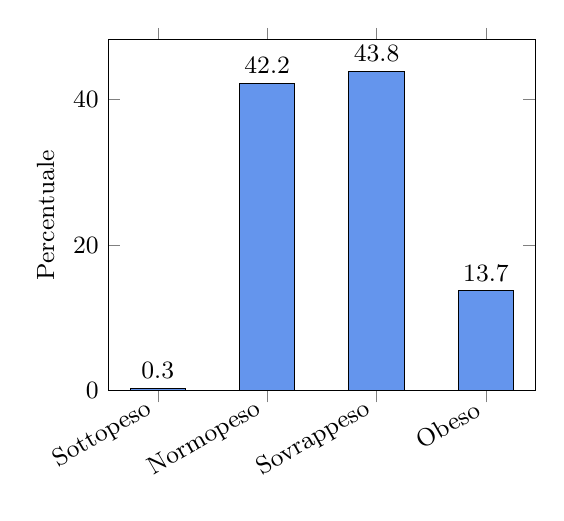
\begin{tikzpicture}[font=\small]
\begin{axis}[ymin=0,
ybar,
xtick=data,
ylabel=Percentuale,
x tick label style={rotate=30,anchor=east},
symbolic x coords={Sottopeso, Normopeso, Sovrappeso, Obeso},
bar width=20pt,enlarge x limits=0.15,nodes near coords,
nodes near coords align={vertical},
]
    \addplot[fill=CornflowerBlue,draw=black]
      coordinates{
	(Sottopeso, .3)
(Normopeso, 42.2)
(Sovrappeso, 43.8)
(Obeso,13.7)
      };
\end{axis}
\end{tikzpicture}

\end{center}

\end{esercizio}

\begin{esercizio}
\label{ese:A.51}
Quattro amici sostengono l'Esame di Stato conseguendo punteggi la cui media aritmetica è~$\np{77,5}/100$.
Se tre di essi hanno conseguito un punteggio, in centesimi, rispettivamente di~70, 76, 80, quale punteggio ha conseguito il quarto studente?
\end{esercizio}
\pagebreak
\begin{esercizio}[Prove Invalsi~2004-2005]
\label{ese:A.52}
La seguente tabella si riferisce alla rilevazione effettuata in una classe prima di un Istituto Tecnico.
\begin{center}
 \begin{tabular}{l*{4}{c}}
\toprule
 & \multicolumn{4}{c}{Scuola media di provenienza}\\
Sesso & Scuola A & Scuola B & Scuola C & Altre scuole\\
\midrule
Maschi & 5 & 3 & 4 & 2 \\
Femmine & 6 & 3 & 4 & 3 \\
\bottomrule
\end{tabular}
\end{center}
Qual è la percentuale di alunni provenienti dalla Scuola B?
\end{esercizio}

\begin{esercizio}[Prove Invalsi~2005-2006]
\label{ese:A.53}
In una classe di~25 alunni, i punteggi (abbreviati in tabella con~$p$) ottenuti in un test di matematica risultano distribuiti come indicato nella seguente tabella.
\begin{center}
 \begin{tabular}{l*{5}{c}}
\toprule
Punteggio & $0 \leq p < 20$ & $20 \leq p < 40$ & $40 \leq p < 60$ & $60 \leq p < 80$ & $80 \leq p \leq~100$ \\
Numero alunni & & & & & \\
\bottomrule
\end{tabular}
\end{center}
Qual è la percentuale di alunni che ha ottenuto un punteggio inferiore a~60?
\end{esercizio}

\begin{esercizio}[Prove Invalsi~2005-2006]
\label{ese:A.54}
Un impiegato ha percepito per i primi~3 mesi dell'anno uno stipendio mensile di \officialeuro~$850$. Nei~9 mesi successivi ha percepito
lo stipendio mensile precedente aumentato di\officialeuro~$200$. Quant'è lo stipendio medio nell'anno di quell'impiegato?
\end{esercizio}

\begin{esercizio}[Prove Invalsi~2005-2006]
\label{ese:A.55}
Nel grafico seguente si riporta l'età dei ragazzi che frequentano una palestra. Qual è la media aritmetica dell'età dei ragazzi
se la distribuzione di frequenza è quella indicata nel grafico?
\begin{center}
 % (c) 2012 Dimitrios Vrettos - d.vrettos@gmail.com
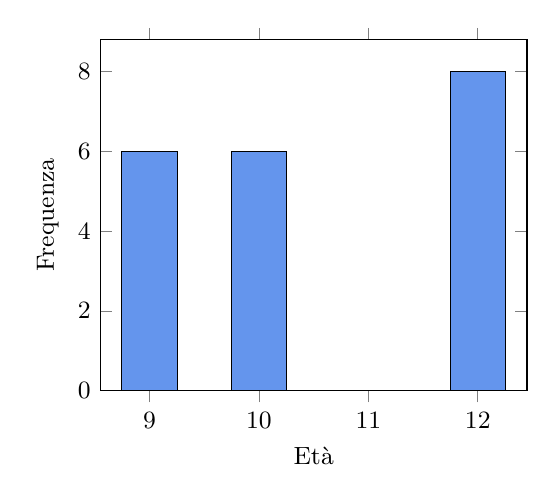
\begin{tikzpicture}[font=\small]

\begin{axis}[ymin=0,
ybar,
ylabel=Frequenza,
xlabel=Età,
bar width=20pt,
enlarge x limits=0.15,]

\addplot[fill=CornflowerBlue,draw=black]
      coordinates{
	(9, 6)
	(10,6)
	(12,8) };
\end{axis}
\end{tikzpicture}

\end{center}
\end{esercizio}
\pagebreak
\begin{esercizio}[Prove Invalsi~2006-2007]
\label{ese:A.56}
I~25 alunni della terza~$C$, dopo aver raccolto i voti conseguiti
nella verifica scritta di matematica, hanno costruito il seguente grafico:
\begin{center}
 % (c) 2012 Dimitrios Vrettos - d.vrettos@gmail.com


\begin{tikzpicture}[x=10mm,y=10mm, x radius=10mm, y radius=10mm]
  \draw (0,0) circle (3);
  \draw[fill=orange] (0,0) -- (0:3) arc (0:14.4:3);
 \draw[fill=brown] (0,0)-- (14.4:3) arc (14.4:57.6:3);
 \draw[fill=green] (0,0)-- (57.6:3) arc (57.6:158.4:3);
\draw[fill=red] (0,0)-- (158.4:3) arc (158.4:273.6:3);
 \draw[fill=blue] (0,0)-- (273.6:3) arc (273.6:316.8:3);
 \draw[fill=olive] (0,0)-- (316.8:3) arc (316.8:345.6:3);
 \draw[fill=lightgray] (0,0)-- (345.6:3) arc (345.6:360:3);

\node[above]  at (0,3) {Voti di Matematica della classe terza $C$};
\begin{scope}[xshift=50mm,
every node/.style={ anchor=center}]
\matrix[matrix of nodes] at (0,0){
\node[fill=orange]{};&Voto 3\\
\node[fill=brown]{};&Voto 4\\
\node[fill=green]{};&Voto 5\\
\node[fill=red]{};&Voto 6\\
\node[fill=blue]{};&Voto 7\\
\node[fill=olive]{};&Voto 8\\
\node[fill=lightgray]{};&Voto 9\\
};
\end{scope}
\begin{scope}[every node/.style={rounded corners, fill=white, draw=black, font=\small}]
\draw(7.2:2.5) node {$4\%$};
\draw(36:2.5) node {$12\%$};
\draw(108:2.5) node {$28\%$};
\draw(216:2.5) node {$32\%$};
\draw(295.2:2.5) node {$12\%$};
\draw(331.2:2.5) node {$8\%$};
\draw(352.8:2.5) node {$4\%$};
\draw(7.2:2.5) node {$4\%$};
\draw(7.2:2.5) node {$4\%$};
\end{scope}
\end{tikzpicture}
\end{center}
Quanti ragazzi hanno conseguito come voto~7?
\begin{multicols}{4}
 \begin{enumeratea}
 \item 12;
 \item 7;
 \item 5;
 \item 3.
\end{enumeratea}
\end{multicols}
\end{esercizio}

\begin{esercizio}
\label{ese:A.57}
La figura indica quanti romanzi leggono gli alunni di una classe in un mese. Quanti sono gli alunni che leggono almeno~2 romanzi?
\begin{center}
 % (c) 2012 Dimitrios Vrettos - d.vrettos@gmail.com

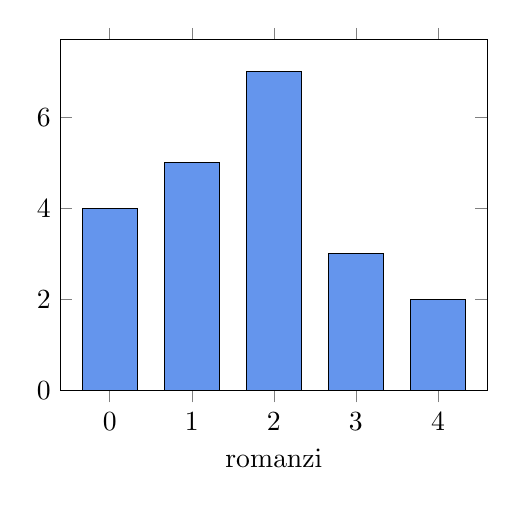
\begin{tikzpicture}
\begin{axis}[ymin=0,
ybar,
xlabel=romanzi,
bar width=20pt,enlarge x limits=0.15
]
    \addplot[fill=CornflowerBlue,draw=black]
      coordinates{
(0,4)
(1,5)
(2,7)
(3,3)
(4,2)
      };
\end{axis}
\end{tikzpicture}
\end{center}
\end{esercizio}
\pagebreak
\begin{esercizio}[Prove Invalsi~2004-2005]
\label{ese:A.58}
Il Ministero dell'Istruzione ha diffuso le seguenti informazioni sul numero di alunni stranieri della scuola italiana
nell'anno scolastico~2003-2004. La tabella riporta solo le~5 nazionalità più numerose.
\begin{center}
 \begin{tabularx}{.95\textwidth}{*{3}{X}}
\toprule
Nazionalità più numerose & Numero di alunni & Percentuale di alunni sul totale degli stranieri \\
\midrule
Albania & $\np{50000}$ & $\np{18,00}\%$ \\
Marocco & $\np{42000}$ & $\np{15,00}\%$ \\
Romania & $\np{28000}$ & $\np{10,00}\%$ \\
Cina    & $\np{16000}$ & $\np{6,00}\%$ \\
Ecuador & $\np{11000}$ & $\np{4,00}\%$ \\
\bottomrule
\end{tabularx}
\end{center}

Cosa si può dedurre da tali dati sugli alunni stranieri di nazionalità russa? Sono~$\ldots$
\begin{enumeratea}
 \item meno di~$\np{11000}$;
 \item sicuramente meno di~400;
 \item una percentuale compresa fra il~4\% e il~18\%;
 \item assenti dalle scuole italiane.
\end{enumeratea}
\end{esercizio}
\begin{esercizio}
\label{ese:A.59}
La tabella mostra la superficie delle varie province del Lazio.
\begin{center}
 \begin{tabular}{l*{5}{c}}
 \toprule
 Provincia & Frosinone & Latina & Rieti & Roma & Viterbo\\
 Superficie ($\unit{km}^2$) & $\np{3240}$& $\np{2251}$& $\np{2749}$& $\np{5352}$& $\np{3612}$\\
 \bottomrule
 \end{tabular}
\end{center}
Quale dei diagrammi riportati sotto descrive graficamente i dati della tabella?
\begin{center}
 % (c) 2012 Dimitrios Vrettos - d.vrettos@gmail.com


\begin{tikzpicture}[scale=.90,x=7mm,y=7mm]
  \draw (0,0) circle (3);
   \draw[fill=orange] (0,0) -- (0:3) arc (0:90:3);
 \draw[fill=brown] (0,0)-- (90:3) arc (90:133.2:3);
  \draw[fill=green] (0,0)-- (133.2:3) arc (133.2:198:3);
\draw[fill=red] (0,0)-- (198:3) arc (198:259.2:3);
\draw[fill=blue] (0,0)-- (259.2:3) arc (259.2:360:3);
\node[above] at (0,3) {1};

\begin{scope}[xshift=50mm]
  \draw (0,0) circle (3);
   \draw[fill=orange] (0,0) -- (0:3) arc (0:36:3);
 \draw[fill=brown] (0,0)-- (36:3) arc (36:64.8:3);
  \draw[fill=green] (0,0)-- (64.8:3) arc (64.8:180:3);
\draw[fill=red] (0,0)-- (180:3) arc (180:324.2:3);
\draw[fill=blue] (0,0)-- (324:3) arc (324:360:3);
\node[above] at (0,3) {2};
\end{scope}

\begin{scope}[xshift=100mm]
  \draw (0,0) circle (3);
   \draw[fill=orange] (0,0) -- (0:3) arc (0:39.6:3);
 \draw[fill=brown] (0,0)-- (39.6:3) arc (39.6:122.4:3);
  \draw[fill=green] (0,0)-- (122.4:3) arc (122.4:194.4:3);
\draw[fill=red] (0,0)-- (194.4:3) arc (194.4:309.6:3);
\draw[fill=blue] (0,0)-- (309.6:3) arc (309.6:360:3);
\node[above] at (0,3) {3};
\end{scope}


\begin{scope}[xshift=25mm, yshift=-50mm]
  \draw (0,0) circle (3);
   \draw[fill=orange] (0,0) -- (0:3) arc (0:68.4:3);
 \draw[fill=brown] (0,0)-- (68.4:3) arc (68.4:115.2:3);
  \draw[fill=green] (0,0)-- (115.2:3) arc (115.2:172.8:3);
\draw[fill=red] (0,0)-- (172.8:3) arc (172.8:284.4:3);
\draw[fill=blue] (0,0)-- (284.4:3) arc (284.4:360:3);
\node[above] at (0,3) {4};
\end{scope}

\begin{scope}[xshift=75mm, yshift=-50mm]
  \draw (0,0) circle (3);
   \draw[fill=orange] (0,0) -- (0:3) arc (0:126:3);
 \draw[fill=brown] (0,0)-- (126:3) arc (126:201.6:3);
  \draw[fill=green] (0,0)-- (201.6:3) arc (201.6:230.4:3);
\draw[fill=red] (0,0)-- (230.4:3) arc (230.4:304.4:3);
\draw[fill=blue] (0,0)-- (304.4:3) arc (304.4:360:3);
\node[above] at (0,3) {5};
\end{scope}

\begin{scope}[xshift=50mm, yshift=35mm]
\matrix[matrix of nodes, every node/.style={anchor=center}]{
\node[fill=orange]{};&Frosinone~~~~&
\node[fill=brown]{};&Latina~~~~&
\node[fill=green]{};&Rieti~~~~&
\node[fill=red]{};&Roma~~~~&
\node[fill=blue]{};&Viterbo\\};

\end{scope}
\end{tikzpicture}
\end{center}

\end{esercizio}

%\newpage
\subsection{Risposte}
\begin{multicols}{2}
 \paragraph{\thechapter.24.}
a)~$6$;\quad b)~$11$, $7$;\quad c)~$75$.

\paragraph{\thechapter.26.} $21$.

\paragraph{\thechapter.27.} $\np{7,1}$.

\paragraph{\thechapter.30.}
a)~$6$;\quad b)~$10$;\quad c)~$89$.

\paragraph{\thechapter.31.} $43$.

\paragraph{\thechapter.32.} $15$.

\paragraph{\thechapter.49.} $15$.

\paragraph{\thechapter.50.} d.
\end{multicols}


\cleardoublepage

